\documentclass[../notes.tex]{subfiles}

\pagestyle{main}
\renewcommand{\chaptermark}[1]{\markboth{\chaptername\ \thechapter\ (#1)}{}}
\setcounter{chapter}{4}

\begin{document}




\chapter{End Quantitative and Intro to Qualitative}
\section{Planar Autonomous Linear Systems}
\begin{itemize}
    \item \marginnote{10/24:}Review of vector fields.
    \item \textbf{Phase diagram}: A diagram that shows the qualitative behavior of an autonomous ordinary differential equation. \emph{Also known as} \textbf{phase portrait}.
    \begin{figure}[h!]
        \centering
        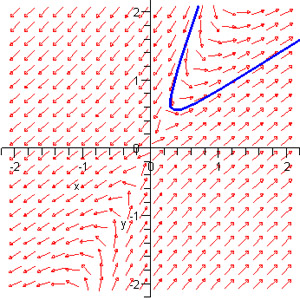
\includegraphics[width=0.4\linewidth]{../ExtFiles/exPhaseDiagram.jpeg}
        \caption{Phase diagram example.}
        \label{fig:exPhaseDiagram}
    \end{figure}
    \begin{itemize}
        \item Consists of a selection of arrows describing, to some extent, a vector field and is often paired with integral curves.
    \end{itemize}
    \item Suppose $\Omega\subset\R^n$ is open.
    \item \textbf{Vector field} (on $\Omega$): A mapping from $\Omega\to\R^n$. \emph{Denoted by} $\bm{X}$.
    \begin{itemize}
        \item Essentially, a vector field assigns to every point of some region a vector; the definition just formalizes this notion.
    \end{itemize}
    \item \textbf{Flow}: A formalization of the idea of the motion of particles in a fluid.
    \begin{itemize}
        \item The solution to the IVP $\dv{y}{t}=X(y)$, $y(0)=x$.
    \end{itemize}
    \item If $X$ is $C^1$, then for all $x\in\Omega$, there exists a unique solution $y$ to the above IVP.
    \item \textbf{Orbit} (of $x$ under $X$): The trajectory $y(t,x)$.
    \begin{itemize}
        \item Recall that the tangent vector to any trajectory at any point coincides with the vector to which $X$ maps that point.
    \end{itemize}
    \item \textbf{Fixed point}: A point $x_0\in\Omega$ such that $X(x_0)=\bar{0}$.
    \begin{itemize}
        \item If $x_0$ is a fixed point, then the trajectory is $y(t)=x_0$.
    \end{itemize}
    \item Today: We will consider flows on vector fields where the dimension is two and our vector field is linear. In particular\dots
    \item Let $A$ be a $2\times 2$ real matrix, and let $X(x)=Ax$.
    \begin{itemize}
        \item In this case, $x_0=0$ is the only fixed point.
        \item The flow is given by the linear differential equation $y'=Ay$, $y(0)=x$. The solution is $y(t)=\e[tA]x$.
    \end{itemize}
    \item Case 1: $A$ has no real eigenvalues.
    \begin{figure}[h!]
        \centering
        \begin{subfigure}[b]{0.32\linewidth}
            \centering
            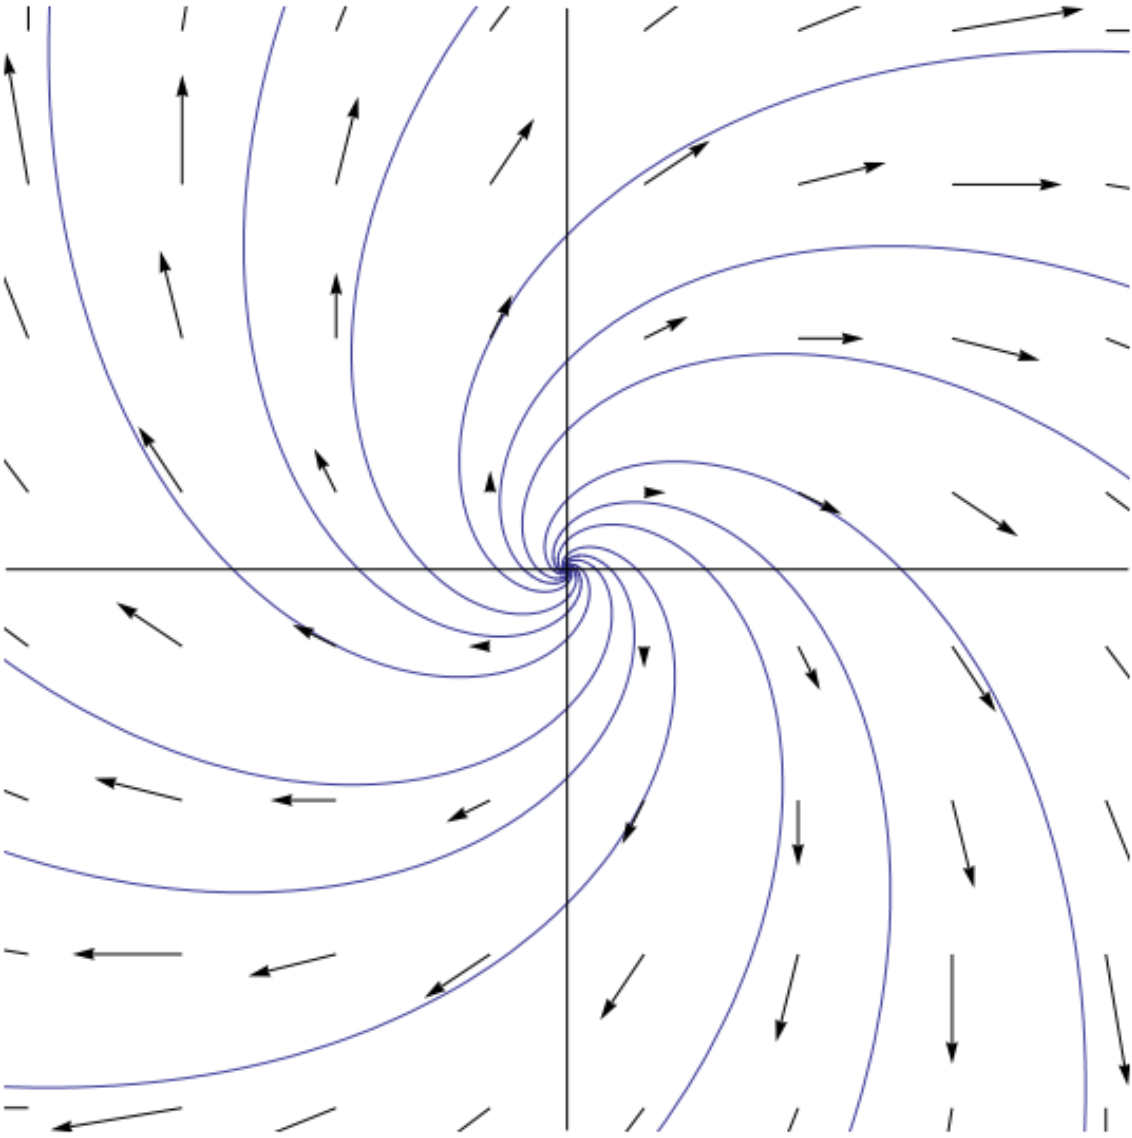
\includegraphics[width=0.8\linewidth]{../ExtFiles/planarComplexa.png}
            \caption{$\sigma>0$.}
            \label{fig:planarComplexa}
        \end{subfigure}
        \begin{subfigure}[b]{0.32\linewidth}
            \centering
            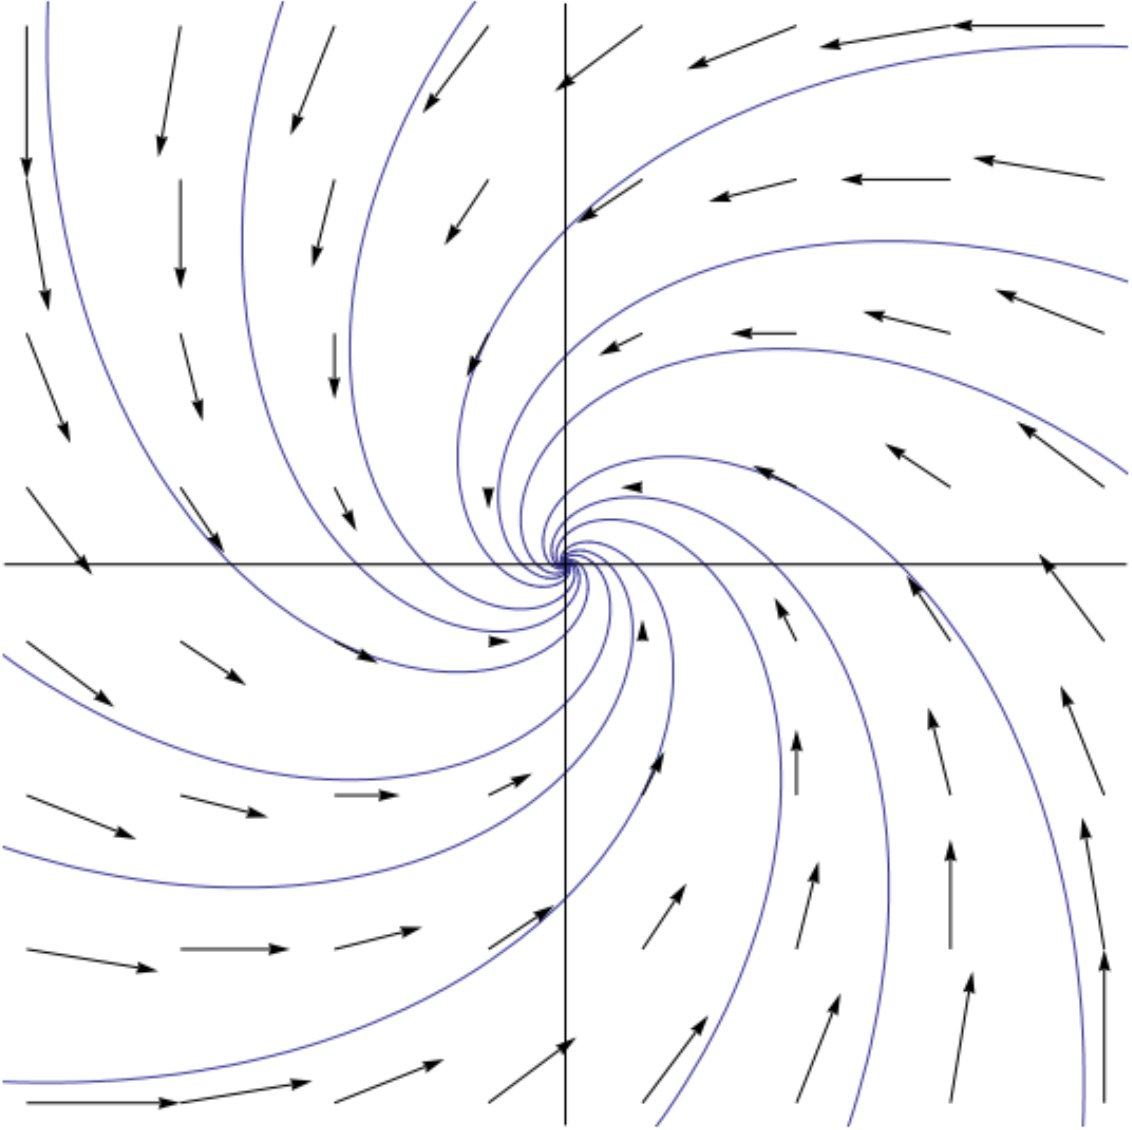
\includegraphics[width=0.8\linewidth]{../ExtFiles/planarComplexb.png}
            \caption{$\sigma<0$.}
            \label{fig:planarComplexb}
        \end{subfigure}
        \begin{subfigure}[b]{0.32\linewidth}
            \centering
            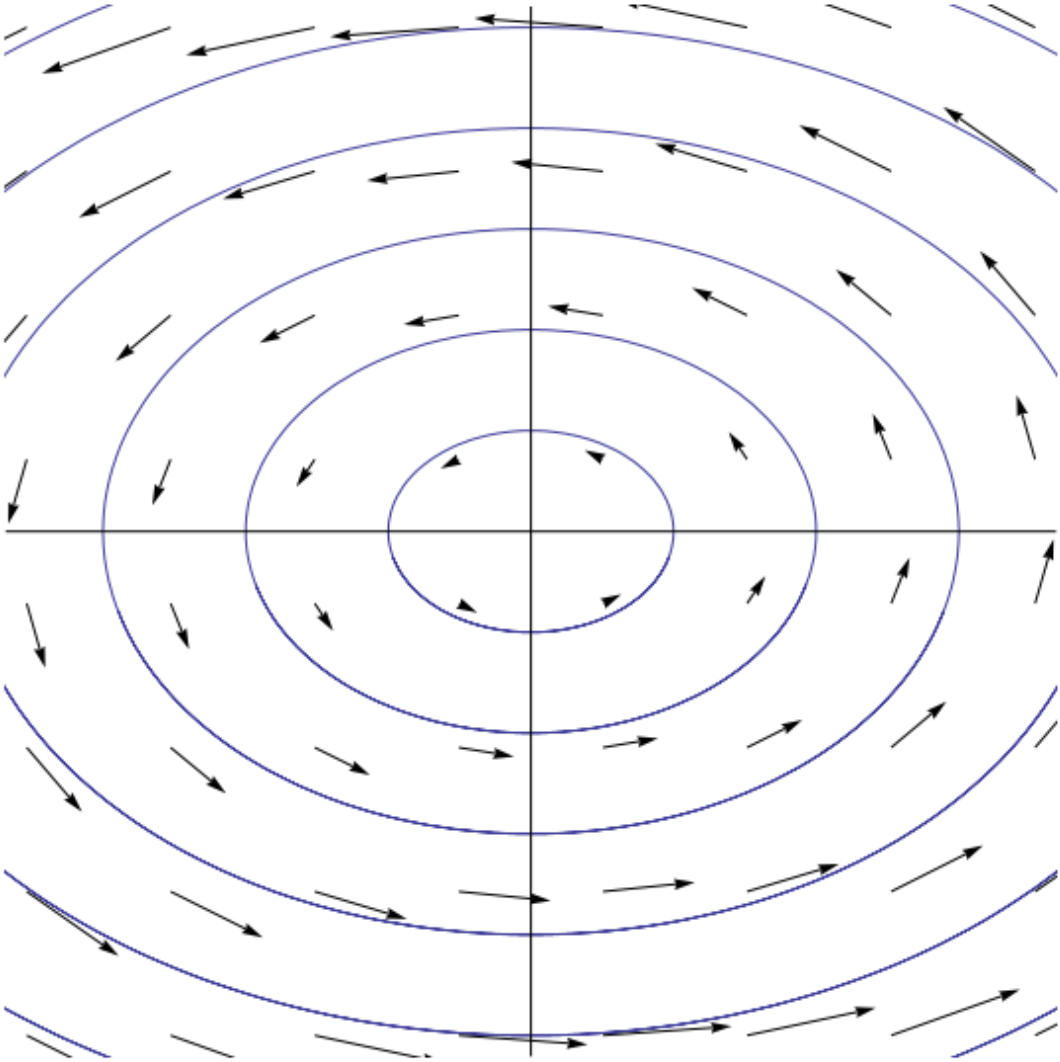
\includegraphics[width=0.8\linewidth]{../ExtFiles/planarComplexc.png}
            \caption{$\sigma=0$.}
            \label{fig:planarComplexc}
        \end{subfigure}
        \caption{Phase diagrams for a planar system with no real eigenvalues.}
        \label{fig:planarComplex}
    \end{figure}
    \begin{itemize}
        \item We know that $\chi_A(z)$ is a real polynomial: $\chi_A(z)=z^2+(\trc A)z+\det A$, and since $A$ is real, both $\trc A$ and $\det A$ are real.
        \item Thus, the eigenvalues appear as conjugate pair, i.e., we may write $\lambda=\sigma+i\beta$ and $\bar{\lambda}=\sigma-i\beta$.
        \begin{itemize}
            \item $\alpha=\gamma=1$ for both eigenvalues.
            \item The eigenvectors must also be complex conjugates.
        \end{itemize}
        \item Distinct eigenvalues imply that $A$ is diagonalizable.
        \item However, this is not what we want because if we use the complex form, then
        \begin{equation*}
            \e[tA] = Q
            \begin{pmatrix}
                \e[t\lambda] & 0\\
                0 & \e[t\bar{\lambda}]\\
            \end{pmatrix}
            Q^{-1}
        \end{equation*}
        \item Indeed, we want to get a real matrix out of $Q,\e[t\Lambda],Q^{-1}$ all complex. We have
        \begin{align*}
            \e[tA]x &= Q
            \begin{pmatrix}
                \e[t(\sigma+i\beta)] & 0\\
                0 & \e[t(\sigma-i\beta)]\\
            \end{pmatrix}
            \underbrace{Q^{-1}x}_z\\
            &= Q
            \begin{pmatrix}
                \e[t(\sigma+i\beta)]z^1\\
                \e[t(\sigma-i\beta)]z^2\\
            \end{pmatrix}\\
            &= z^1\e[t(\sigma+i\beta)]v+z^2\e[t(\sigma-i\beta)]\bar{v}
        \end{align*}
        \item Since $y(0)=x=z^1v+z^2\bar{v}\in\R^2$ (i.e., $z^1v+z^2v$ is \emph{real}), we know that it is equal to its complex conjugate. This tells us that
        \begin{align*}
            z^1v+z^2\bar{v} &= \bar{z^1}\bar{v}+\bar{z^2}v\\
            z^1 &= \bar{z^2}
        \end{align*}
        \item It follows that
        \begin{align*}
            y(t) &= \e[tA]x\\
            &= z^1\e[t(\sigma+i\beta)]v+\bar{z^1}\e[t(\sigma-i\beta)]\bar{v}\\
            &= z^1\e[t(\sigma+i\beta)]v+\overline{z^1\e[t(\sigma+i\beta)]v}\\
            &= 2\Ree(z^1\e[t(\sigma+i\beta)]v)\\
            &= 2\Ree(z^1\e[\sigma t](\cos(\beta t)+i\sin(\beta t))(v_1+iv_2))\\
            &= 2\Ree(z^1\e[\sigma t](\cos(\beta t)v_1+i\cos(\beta t)v_2+i\sin(\beta t)v_1-\sin(\beta t)v_2))\\
            &= 2\e[\sigma t]\cos(\beta t)\cdot\Ree(z^1v)-2\e[\sigma t]\sin(\beta t)\cdot\Imm(z^1v)
        \end{align*}
        \item How do we get from the second-to-last line to the last line above??
        \item Suppose $\sigma\neq 0$. Then
        \begin{equation*}
            x \mapsto
            \begin{pmatrix}
                \Ree(z^1v)\\
                \Imm(z^1v)\\
            \end{pmatrix}
        \end{equation*}
        is a real linear transformation on $\R^2$.
        \item It follows that the trajectories are just spirals in the complex plane.
        \item If $\sigma>0$, then the spiral repels from the origin. If $\sigma<0$, then the spiral attracts to the origin. If $\sigma=0$, we get an ellipse.
        \item Therefore, we have completely classified equations of the form
        \begin{equation*}
            \begin{pmatrix}
                y^1\\
                y^2\\
            \end{pmatrix}'
            =
            \begin{pmatrix}
                y^2\\
                -\omega^2y^1\\
            \end{pmatrix}
        \end{equation*}
    \end{itemize}
    \item Case 2: $A$ has real eigenvalues and \emph{is} diagonalizable.
    \begin{figure}[h!]
        \centering
        \begin{subfigure}[b]{0.32\linewidth}
            \centering
            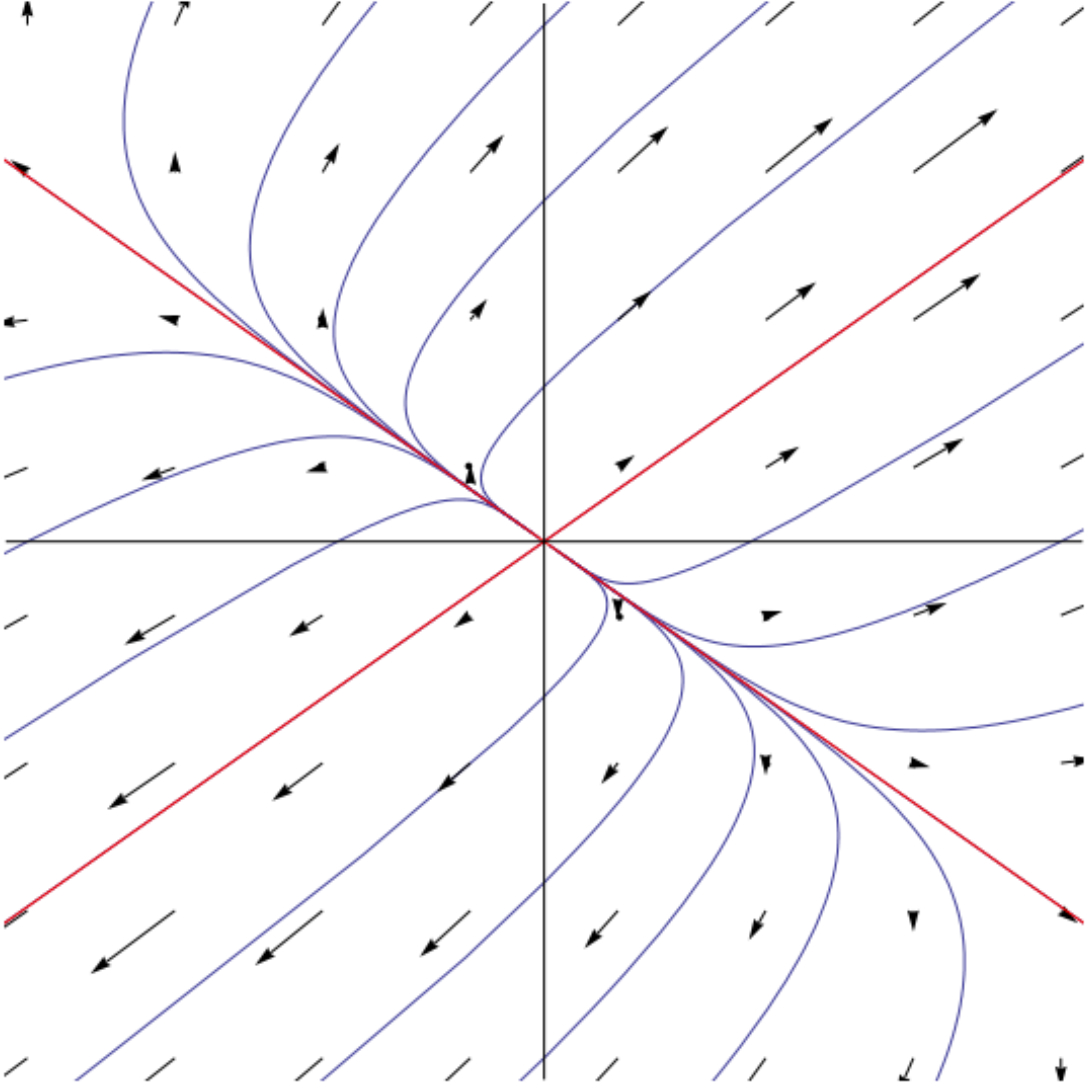
\includegraphics[width=0.8\linewidth]{../ExtFiles/planarRealDiaga.png}
            \caption{$\lambda_1,\lambda_2>0$.}
            \label{fig:planarRealDiaga}
        \end{subfigure}
        \begin{subfigure}[b]{0.32\linewidth}
            \centering
            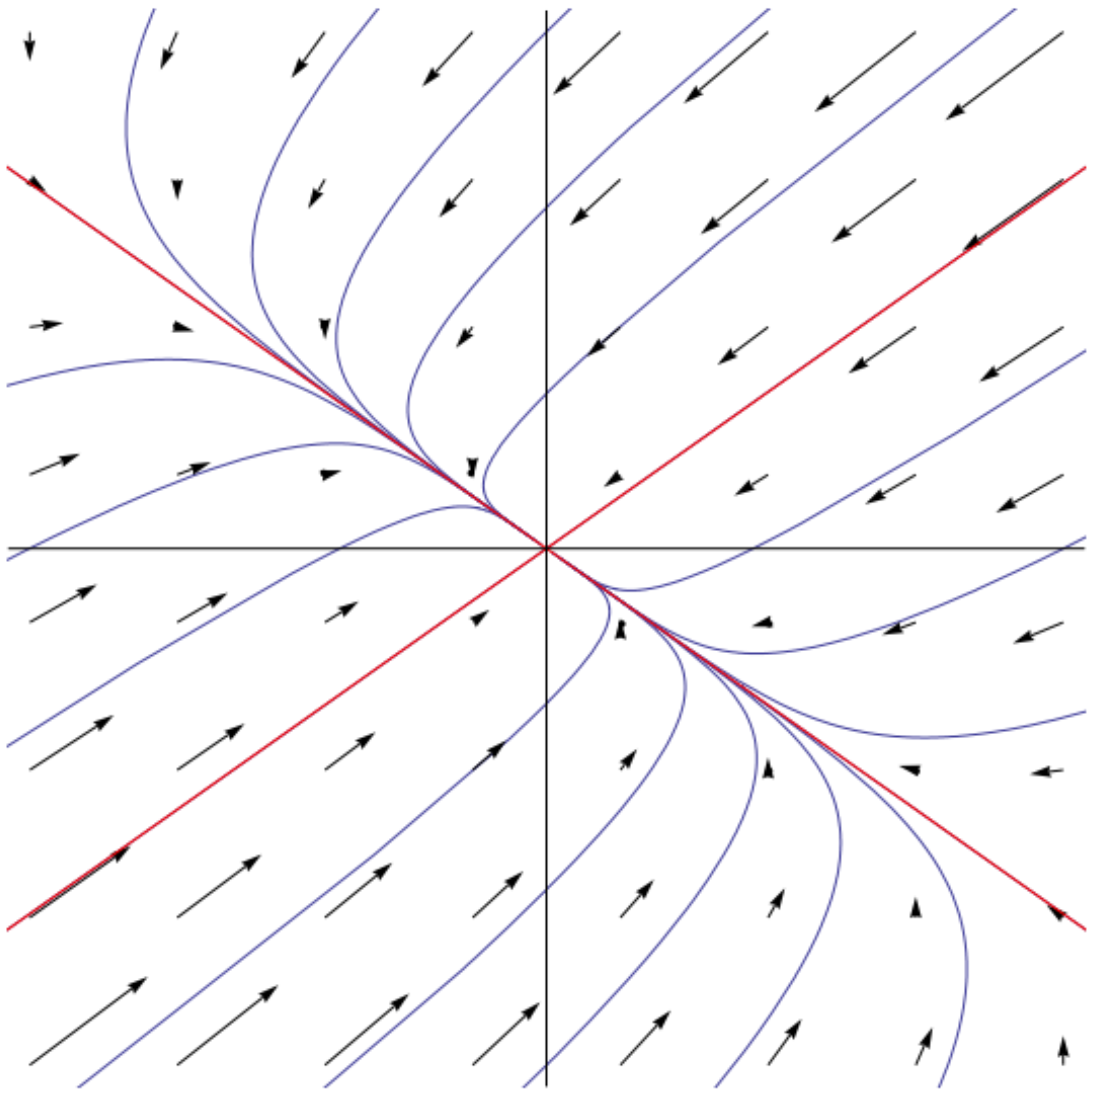
\includegraphics[width=0.8\linewidth]{../ExtFiles/planarRealDiagb.png}
            \caption{$\lambda_1,\lambda_2<0$.}
            \label{fig:planarRealDiagb}
        \end{subfigure}
        \begin{subfigure}[b]{0.32\linewidth}
            \centering
            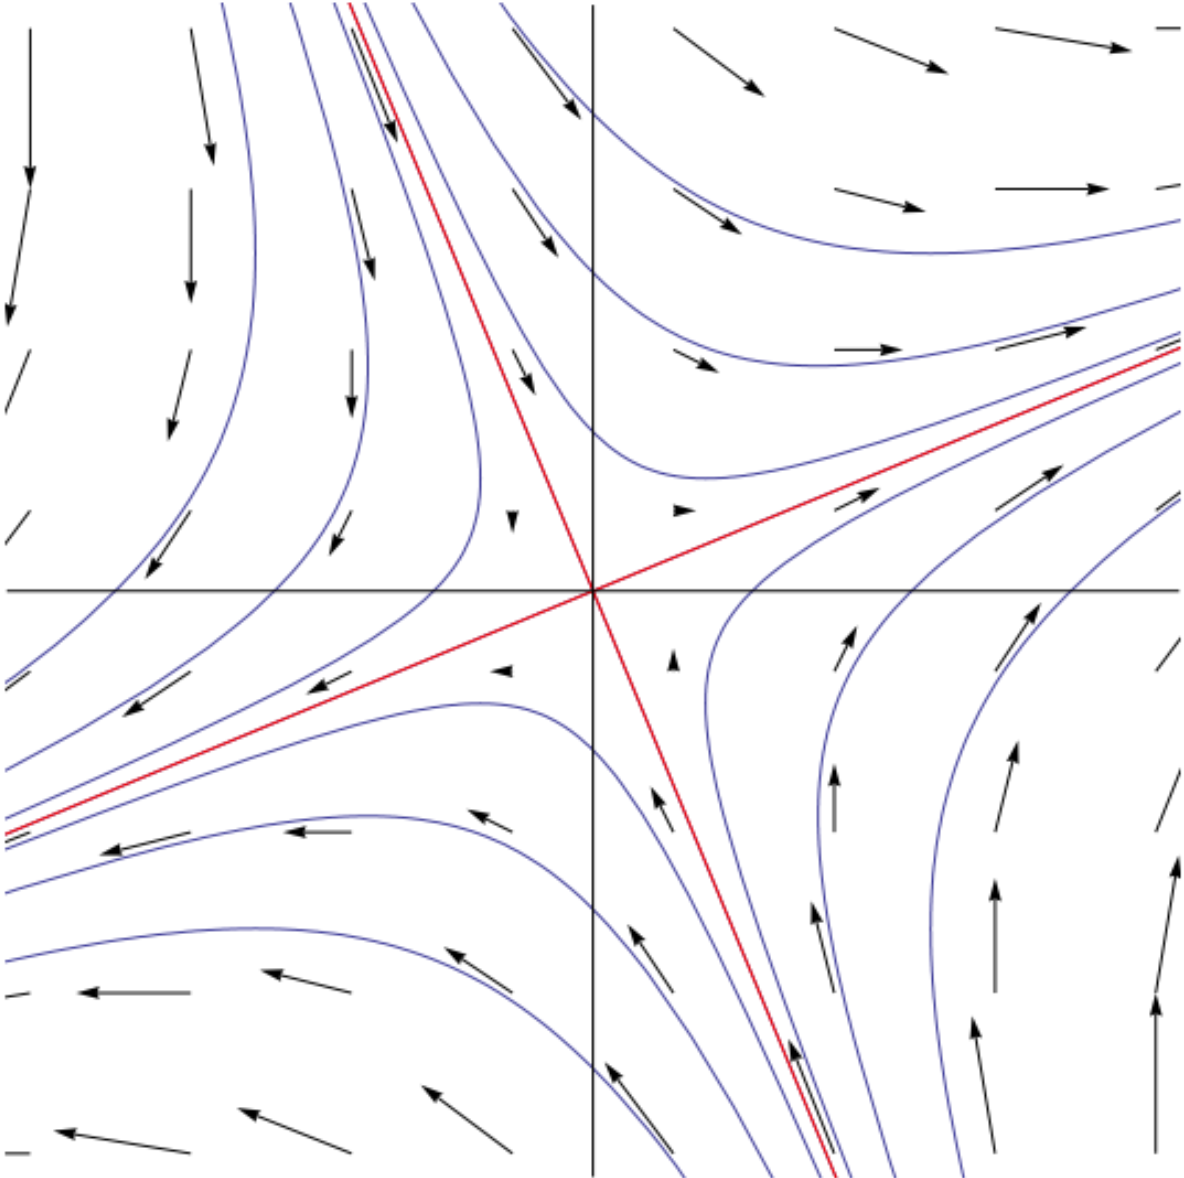
\includegraphics[width=0.8\linewidth]{../ExtFiles/planarRealDiagc.png}
            \caption{$\lambda_1<0<\lambda_2$ (WLOG).}
            \label{fig:planarRealDiagc}
        \end{subfigure}
        \caption{Phase diagrams for a diagonalizable planar system with real eigenvalues.}
        \label{fig:planarRealDiag}
    \end{figure}
    \begin{itemize}
        \item Suppose $\lambda_1,\lambda_2\in\R$ have corresponding linearly independent eigenvectors $v_1,v_2$.
        \item If we choose $v_1,v_2$ to be our basis, then
        \begin{equation*}
            \e[tA] = Q
            \begin{pmatrix}
                \e[t\lambda_1] & 0\\
                0 & \e[t\lambda_2]\\
            \end{pmatrix}
            Q^{-1}
        \end{equation*}
        where $
            Q =
            \begin{pmatrix}
                v_1 & v_2\\
            \end{pmatrix}
        $.
        \item Thus, as before, the solution may be expressed in the following form, where $z=Q^{-1}x$.
        \begin{equation*}
            y(t) = \e[tA]x
            = \e[\lambda_1t]z^1v_1+\e[\lambda_2t]z^2v_2
        \end{equation*}
        \item Moving forward, it will be convenient to work in the $v_1,v_2$ basis. We divide into three subcases ($\lambda_1,\lambda_2>0$ [Figure \ref{fig:planarRealDiaga}], $\lambda_1,\lambda_2<0$ [Figure \ref{fig:planarRealDiagb}], and WLOG $\lambda_1<0<\lambda_2$ [Figure \ref{fig:planarRealDiagc}]).
        \begin{enumerate}
            \item Notice that
            \begin{equation*}
                \e[\lambda_2t] = \e[(\lambda_2/\lambda_1)(\lambda_1t)]
            \end{equation*}
            i.e., $\e[\lambda_2t]$ is a power of $\e[\lambda_1t]$. Thus, when the signs are the same, we get a power function $v_2=v_1^{\lambda_2/\lambda_1}$.
            \begin{itemize}
                \item Both subspaces $v_1,v_2$ are unstable here.
            \end{itemize}
            \item If $\lambda_1,\lambda_2<0$, then we have the same trajectories, but they're all attracted to the origin instead of repelled.
            \begin{itemize}
                \item Both subspaces $v_1,v_2$ are stable here.
            \end{itemize}
            \item When both eigenvalues have different signs, we are considering power functions of a negative power.
            \begin{itemize}
                \item The stable subspace is $v_2$ and the unstable subspace is $v_1$ here.
            \end{itemize}
        \end{enumerate}
    \end{itemize}
    \item Case 3: $A$ has real eigenvalues and \emph{is not} diagonalizable.
    \begin{figure}[h!]
        \centering
        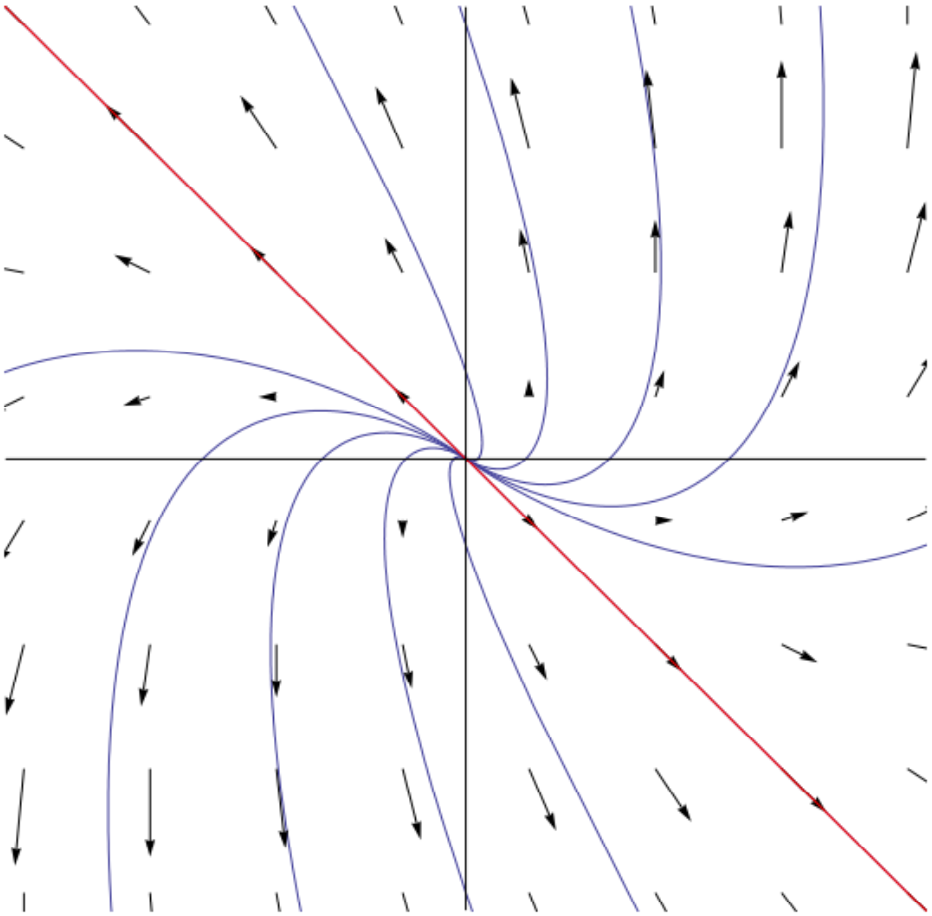
\includegraphics[width=0.256\linewidth]{../ExtFiles/planarRealNon.png}
        \caption{Phase diagrams for a nondiagonalizable planar system with real eigenvalues.}
        \label{fig:planarRealNon}
    \end{figure}
    \begin{itemize}
        \item In this case, the matrix exponential is given by
        \begin{equation*}
            \e[tA] = Q
            \begin{pmatrix}
                \e[t\lambda] & t\e[t\lambda]\\
                0 & \e[t\lambda]\\
            \end{pmatrix}
            Q^{-1}
        \end{equation*}
        \item The solution is given by
        \begin{equation*}
            \e[tA]x = (z^1\e[t\lambda]+z^2t\e[t\lambda])v+z^2\e[t\lambda]u
        \end{equation*}
        where $Q^{-1}x=z$ again.
        \item In graphing, note that here we have (a distorted version of) the form $y=x\pm x\log x$:
        \begin{align*}
            y &= (z^1\e[t\lambda]+z^2t\e[t\lambda])\hat{\imath}+z^2\e[t\lambda]\hat{\jmath}
            \intertext{Define $x:=\e[t\lambda]$. Then $t=\lambda^{-1}\ln x$. Substituting, we have}
            &= (z^1x+z^2(\lambda^{-1}\ln x)x)\hat{\imath}+z^2x\hat{\jmath}\\
            &= (z^1x+z^2\lambda^{-1}x\ln x)\hat{\imath}+z^2x\hat{\jmath}
        \end{align*}
        \item When $\lambda>0$, the whole space is unstable. Thus, the phase diagram is tangent to the origin.
        \item When $\lambda<0$, the trajectories take the same form but this time are attracted to zero. In this case, the whole space is stable.
    \end{itemize}
    \item We can take $x_1$ to $x_2$ iff they are in the same orbit. Conclusion: Orbits never cross.
    \item Takeaway: You should be able to compute the eigenvalues and eigenvectors and sketch these graphs.
    \item Shao will post lecture notes after today's lecture!
    \item Next lecture: The final explicitly solveable case, which is the driven harmonic oscillator.
\end{itemize}



\section{Driven Harmonic Oscillator and Resonance}
\begin{itemize}
    \item \marginnote{10/26:}We are interested in the 2nd order constant coefficient equation
    \begin{equation*}
        x''+\mu x'+\omega_0^2x = H_0\e[i\omega t]
    \end{equation*}
    where $\mu\geq 0$ and $\omega_0,\omega>0$.
    \item Two cases where this ODE arises:
    \begin{figure}[h!]
        \centering
        \footnotesize
        \begin{subfigure}[b]{0.35\linewidth}
            \centering
            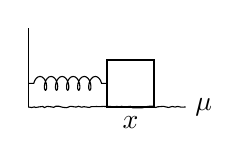
\begin{tikzpicture}
                \draw (0,1) -- (0,0);
                \draw [decorate,decoration={random steps,segment length=1pt,amplitude=0.3pt}] (0,0) -- (2,0) node[right]{$\mu$};
                \draw [decorate,decoration={coil,segment length=4pt,pre length=2pt}] (0,0.3) -- ++(1,0);
    
                \draw [semithick] (1,0) node[xshift=3mm,yshift=-2mm]{$x$} rectangle (1.6,0.6);
            \end{tikzpicture}
            \caption{A driven harmonic oscillator.}
            \label{fig:drivenHOorigina}
        \end{subfigure}
        \begin{subfigure}[b]{0.35\linewidth}
            \centering
            \begin{circuitikz}
                \draw (0,0)
                    to[L,l_=L] (2,0)
                    to[C,l_=C] (2,1)
                    to[R,l_=R] (0,1)
                    to[battery1,l_=$V(t)$] (0,0)
                ;
            \end{circuitikz}
            \caption{An RLC circuit.}
            \label{fig:drivenHOoriginb}
        \end{subfigure}
        \caption{Origins of the driven harmonic oscillator equation.}
        \label{fig:drivenHOorigin}
    \end{figure}
    \begin{enumerate}
        \item The driven harmonic oscillator.
        \begin{itemize}
            \item Consider a mass on a spring.
            \item The extent of friction between the mass point and the surface is described by $\mu$.
            \item The oscillation is periodically driven by a force of magnitude $H_0\cos\omega t$.
        \end{itemize}
        \item RLC circuit.
        \begin{itemize}
            \item R is resistance, L is inductance, C is capacitance.
            \item We have the laws
            \begin{align*}
                LI'_L(t) &= V_L&
                CV_C'(t) &= I_C&
                I_R(t) &= V_R(t)/R
            \end{align*}
            \begin{itemize}
                \item Left: Self-inductance.
                \item Right: Ohm's law.
            \end{itemize}
            \item Combining them with Kirchhoff's laws
            \begin{align*}
                I(t) &= I_R = I_C = I_L&
                V(t) &= V_R+V_L+V_C
            \end{align*}
            we get the RLC circuit equation
            \begin{equation*}
                LI''+RI'+\frac{I}{C} = V'(t)
            \end{equation*}
            \item The most interesting cases is when we have a source of alternating current of frequency $\omega$. In this case, $V(t)=V_0\cos\omega t$ or, in the complex case, $V(t)=V_0\e[i\omega t]$. This yields the complex equation
            \begin{equation*}
                I''+\frac{R}{L}I'+\frac{1}{LC}I = \frac{i\omega V_0}{L}\e[i\omega t]
            \end{equation*}
            \item Here, the friction coefficient $\mu=R/L$ and the frequency is $\omega_0=\sqrt{1/LC}$.
        \end{itemize}
    \end{enumerate}
    \item Recall that we want to solve the following ODE.
    \begin{equation*}
        x''+\mu x'+\omega_0^2x = H_0\e[i\omega t]
    \end{equation*}
    \begin{itemize}
        \item The homogeneous linear equation $x''+\mu x'+\omega_0^2x=0$ is well-understood, i.e., we can find all of the \emph{homogeneous} solutions to the above equation.
        \item Thus, to solve the above inhomogeneous equation, we just have to find a particular solution.
    \end{itemize}
    \item WLOG let $\omega>0$.
    \item From the homework, a particular solution $x_p(t)$ with initial condition $x_p(0)=x_p'(0)=\mu=0$ can be obtained from the Duhamel formula as follows.
    \begin{equation*}
        x_p(t) = H_0\int_0^t\frac{\sin\omega_0(t-\tau)}{\omega_0}\e[i\omega\tau]\dd\tau
    \end{equation*}
    \begin{itemize}
        \item Substituting
        \begin{equation*}
            \sin\theta = \frac{\e[i\theta]-\e[-i\theta]}{2i}
        \end{equation*}
        into the above allows us to evaluate it.
        \item In particular, it follows that
        \begin{equation*}
            x_p(t) =
            \begin{cases}
                \displaystyle\frac{H_0}{\omega_0^2-\omega^2}\left( \e[i\omega t]-\cos\omega_0t-\frac{i\omega}{\omega_0}\sin\omega_0t \right) & \omega\neq\omega_0\\
                \displaystyle -\frac{iH_0}{2\omega_0}\left( t\e[i\omega_0t]-\frac{\sin\omega_0t}{\omega_0} \right) & \omega=\omega_0
            \end{cases}
        \end{equation*}
        \begin{itemize}
            \item We compute the $\omega=\omega_0$ case using L'H\^{o}pital's rule to analyze the $\omega\neq\omega_0$ case as $\omega\to\omega_0$.
        \end{itemize}
        \item If we pump in energy at the same point that we have deviation ($\omega=\omega_0$), then the amplitude of oscillation goes to $\infty$.
        \begin{itemize}
            \item Practically, when $\omega\approx\omega_0$, the long-time behavior of the driven oscillator will be very much like a growing oscillator.
            \item Eventually, the amplitude will be approximately $(\omega-\omega_0)^{-1}$.
        \end{itemize}
    \end{itemize}
    \item \textbf{Resonance catastrophe}: Inputing energy into a system at its natural frequency, causing the total energy to grow until a mechanical failure occurs.
    \begin{itemize}
        \item This is what happened at the Millenium Bridge in London; synchronized footsteps caused the bridge to shake really wildly.
    \end{itemize}
    \item If $\mu>0$, there will be a particular solution of the form
    \begin{equation*}
        x_p(t) = A(\omega)H_0\e[i\omega t]
    \end{equation*}
    \begin{itemize}
        \item From HW1, we have three cases when $\mu>0$: $0<\mu<2\omega_0$, $\mu=2\omega_0$, and $\mu>2\omega_0$. These are just the three cases of the characteristic polynomial??
        \item Substituting the proposed form of the particular solution into the differential equation, we get
        \begin{align*}
            x_p''+\mu x_p'+\omega_0^2x_p &= H_0\e[i\omega t]\\
            (-\omega^2+i\omega\mu+\omega_0^2)H_0A(\omega)\e[i\omega t] &= H_0\e[i\omega t]\\
            (-\omega^2+i\omega\mu+\omega_0^2)A(\omega) &= 1\\
            A(\omega) &= \frac{1}{\omega_0^2-\omega^2+i\mu\omega}
        \end{align*}
        \item In theory, we avoid the resonance catastrophe in this case. In practice, however, when $\omega\to 0$, we still run into issues.
        \item For mass point:
        \begin{equation*}
            |H_0A(\omega)| = \frac{|H_0|}{\sqrt{(\omega^2-\omega_0^2)^2+\mu^2\omega^2}}
        \end{equation*}
        \begin{itemize}
            \item The norm $|H_0A(\omega)|$ is maximized when $\omega_r=\sqrt{\omega_0^2+\mu^2/2}$.
            \item $\omega_r\to\omega_0$ implies $\mu\to 0$??
        \end{itemize}
        \item As for the argument/angle,
        \begin{equation*}
            \arg(H_0A(\omega)) = \arg H_0+\arg A(\omega)
        \end{equation*}
        \item We consider $\omega:0\to\omega_0\to+\infty$.
        \begin{itemize}
            \item When $\omega=0$, the complex amplitude is $1/\omega_0^2$ so it's a real number in the complex plane.
            \item If $\omega$ is increased a bit, we get the reciprocal of a complex number. Norm is reciprocal, argument is negative.
            \item For $\omega=\omega_0$, we have a purely imaginary number.
            \item As $\omega\to\infty$, the argument approaches $-\pi$??
            \item Showing the shape of the norm and the argument with respect to $\omega$. This allows us to completely describe the resonance phenomena.
        \end{itemize}
    \end{itemize}
    \item For the RLC circuit, the discussion is a bit different.
    \begin{itemize}
        \item The external voltage $V(t)=V_0\e[i\omega t]$. Thus, $V'(t)=iV_0\omega\e[i\omega t]$.
        \item Here,
        \begin{equation*}
            x_p(t) = \frac{iV_0\omega\e[i\omega t]}{\omega_0^2-\omega^2+iR\omega/L}
        \end{equation*}
        \item Look at the complex amplitude.
        \begin{itemize}
            \item Multiply the numerator and denominator by the inductance $L$ to get
            \begin{equation*}
                x_p(t) = \frac{iV_0\omega L\e[i\omega t]}{L\omega_0^2-L\omega^2+iR\omega}
            \end{equation*}
            \item Then,
            \begin{equation*}
                \text{Norm} = \frac{V_0L}{\sqrt{R^2+\left( \frac{1}{C\omega}-\frac{\omega}{L} \right)^2}}
            \end{equation*}
            \item For an RLC circuit, the resistance does not affect the resonance frequency.
            \begin{equation*}
                \omega_r = \sqrt{\frac{1}{LC}} = \omega_0
            \end{equation*}
            \item If you have an external source of voltage, then you can vary the capacity of your circuit to ensure that the voltage will be maximized at a given frequency. We can tune our circuit to a very specific resonance frequency (this is used to filter our radio stations). The RLC circuit is only observable when the resonance coincides with the external resonance.
        \end{itemize}
    \end{itemize}
    \item There will be a bonus problem which is a PDE describing the vibration of a string.
    \begin{itemize}
        \item Suppose we have a string with fixed endpoints, and suppose it is undergoing a small vibration.
        \item Deviation from the equilibrium is described by a function $u(x,t)$.
        \item The simplest equation we can derive is the 1D linear wave equation
        \begin{equation*}
            \pdv[2]{u}{t}-\frac{1}{c^2}\pdv[2]{u}{x} = f(x,t)
        \end{equation*}
        \begin{itemize}
            \item $c$ is the speed of the wave.
            \item $f(x,t)$ is the given external force.
        \end{itemize}
        \item We can show that when $f(x,t)=0$, then the vibration of the string is the linear supposition of infinitely many standing waves.
        \begin{equation*}
            u(x,t) = \sum_{k=1}^\infty a_k\e[\frac{\pi kt}{\ell}]\sin\frac{k\pi}{\ell}x
        \end{equation*}
        \begin{itemize}
            \item There are $k-1$ nodes in the string. These are called standing waves.
        \end{itemize}
        \item If you drive it with frequency
        \begin{equation*}
            f(x,t) = \cos\omega t\sin\frac{k\pi}{\ell}x
        \end{equation*}
        you encounter the resonance catastrophe.
    \end{itemize}
    \item We are interested in the driven harmonic oscillator because it describes the vibrations, even of PDEs.
    \item This concludes our discussion of explicitly solvable differential equations.
    \item Those that are solvable by power series require complex analysis.
    \item Starting this Friday, we will talk about the qualitative theory of differential equations.
    \item Cauchy-Lipschitz this Friday.
    \item Next week: Continuous dependence on initial values and differentiation with respect to the parameter of this equation.
    \item After this, we will be able to compute classical examples in the theory of perturbations.
    \item We will be able to solve the procession of Mercury problem (which was the first experimental verification of general relativity).
\end{itemize}



\section{Qualitative Theory of ODEs}
\begin{itemize}
    \item \marginnote{10/28:}First issue: Uniqueness --- we want to be able to talk about \emph{the} solution to the IVP.
    \item We will be considering the IVP $y'(t)=f(t,y)$, $y(t_0)=y_0$ for $y(t)$ an $\R^n$-valued function.
    \item To embed our rough outline of the Cauchy-Lipschitz theorem into analysis, we start with metric spaces.
    \item \textbf{Metric space}: A set and a metric. \emph{Denoted by} $\bm{(X,d)}$.
    \item \textbf{Metric}: A function from $X\times X\to[0,+\infty)$ that satisfies the following three axioms. \emph{Denoted by} $\bm{d}$.
    \begin{enumerate}
        \item $d(x,y)=d(y,x)$.
        \item $d(x,y)\geq 0$ and $d(x,y)=0$ iff $x=y$.
        \item Triangle inequality: $d(x,z)\leq d(x,y)+d(y,z)$.
    \end{enumerate}
    \item Examples:
    \begin{enumerate}
        \item $\R^n$ with $d(x,y)=\norm{x-y}=\sqrt{\sum_{j=1}^n|x^j-y^j|^2}$.
        \item Continuous functions $y:[a,b]\to\R^n$ with $d(y_1,y_2)=\norm{y_1-y_2}=\sup_{t\in[a,b]}|y_1(t)-y_2(t)|$.
    \end{enumerate}
    \item In Euclidean spaces, we have \textbf{completeness}.
    \item \textbf{Cauchy} (sequence): A sequence $\{x_n\}\subset X$ such that for all $\varepsilon>0$, there exists $N\geq 0$ such that $d(x_m,x_n)<\varepsilon$ for all $m,n>N$.
    \item \textbf{Convergent} (sequence): A sequence $\{x_n\}\subset X$ for which there exists $x\in X$ such that
    \begin{equation*}
        \lim_{n\to\infty}d(x,x_n)=0
    \end{equation*}
    \item \textbf{Complete} (metric space): A metric space $(X,d)$ such that every Cauchy sequence is convergent.
    \item Theorem (Banach fixed point theorem): Let $(X,d)$ be a complete metric space and let $\Phi:X\to X$ be a function for which there exists $q\in(0,1)$ such that for all $x,y\in X$,
    \begin{equation*}
        d(\Phi(x),\Phi(y)) \leq q\cdot d(x,y)
    \end{equation*}
    Then there exists a unique $x\in X$ such that $x=\Phi(x)$.
    \begin{proof}
        We first construct the desired fixed point $x$.\par
        Pick any $x_0\in X$. Inductively define $\{x_n\}$ by $x_{n+1}=\Phi(x_n)$, starting from $n=0$. We will now show that $\{x_n\}$ is a Cauchy sequence. As a lemma, we will prove by induction that
        \begin{equation*}
            d(x_j,x_{j+1}) \leq q^j\cdot d(x_0,x_1)
        \end{equation*}
        for all $j\in\N_0$. For the base case $j=0$, equality evidently holds. Now suppose inductively that we have proven that $d(x_j,x_{j+1})\leq q^j\cdot d(x_0,x_1)$; we want to prove the claim for $j+1$. But we have that
        \begin{align*}
            d(x_{j+1},x_{j+2}) &= d(\Phi(x_j),\Phi(x_{j+1}))\\
            &\leq q\cdot d(x_j,x_{j+1})\\
            &\leq q\cdot q^j\cdot d(x_0,x_1)\\
            &= q^{j+1}\cdot d(x_0,x_1)
        \end{align*}
        as desired.\par
        It follows that
        \begin{align*}
            d(x_n,x_{n+m}) &\leq \sum_{k=0}^{m-1}d(x_{n+k},x_{n+k+1})\tag*{Triangle inequality}\\
            &\leq \sum_{k=0}^{m-1}q^{n+k}\cdot d(x_0,x_1)\tag*{Lemma}\\
            &= q^n(1+q+\cdots+q^{m-1})\cdot d(x_0,x_1)\\
            &< q^n(1+q+\cdots+q^{m-1}+\cdots)\cdot d(x_0,x_1)\\
            &= \frac{q^n}{1-q}\cdot d(x_0,x_1)
        \end{align*}
        It follows that the above term will converge to zero as $n\to\infty$, so $\{x_n\}$ is a Cauchy sequence and there exists an $x$ such that $x_n\xrightarrow{d}x$.\par\smallskip
        We now prove that $x$ is a fixed point of $\Phi$, i.e., that $\Phi(x)=x$. We have that
        \begin{align*}
            d(x,\Phi(x)) &\leq d(x,x_n)+d(x_n,\Phi(x_n))+d(\Phi(x_n),\Phi(x))\\
            &\leq d(x,x_n)+d(x_n,x_{n+1})+q\cdot d(x_n,x)\\
            &= (1+q)\cdot d(x,x_n)+d(x_n,x_{n+1})
        \end{align*}
        where the first term converges since $\{x_n\}$ is convergent and the second term converges since $\{x_n\}$ is Cauchy. Thus, $d(x,\Phi(x))\to 0$ as $n\to\infty$, so $x=\Phi(x)$, as desired.\par
        Lastly, we prove that $x$ is unique. Suppose that there exists $y\in X$ such that $y=\Phi(y)$. Then
        \begin{equation*}
            d(x,y) = d(\Phi(x),\Phi(y))
            \leq q\cdot d(x,y)
        \end{equation*}
        It follows that $d(x,y)\leq q^n\cdot d(x,y)$, i.e., that $d(x,y)\to 0$ as $n\to\infty$. Therefore, we must have that $d(x,y)=0$, from which it follows that $x=y$, as desired.
    \end{proof}
    \item Notes on the Banach fixed point theorem.
    \begin{itemize}
        \item $\Phi$ is a \textbf{contraction}.
        \item Shao gives the example of crumpling a sheet of paper (more specifically, dropping a map of a park in that park; a point coincides).
    \end{itemize}
    \item Example: Fixed point of the cosine function.
    \begin{itemize}
        \item Define $\{x_n\}$ by $x_{n+1}=\cos x_n$. If $x_0\in\R$, then $x_1\in[-1,1]$ and $x_2\in[\cos 1,1]$.
        \item Thus, while cosine is not a contraction on the real numbers ($\cos'(-\pi/2)=1$, for example), we can show that $\cos:[\cos 1,1]\to[\cos 1,1]$ is a contraction: If $x,y\in[\cos 1,1]$, then
        \begin{align*}
            |\cos x-\cos y| &= \left| \int_y^x-\sin t\dd{t} \right|\\
            &\leq |x-y|\sup_{t\in[\cos 1,1]}|\sin t|\\
            &\leq (\sin 1)|x-y|
        \end{align*}
        \item Thus, cosine has a fixed point at the intersection of $y=\cos x$ and $y=x$ of approximate value 0.739\dots
        \item Overall, this is a pretty bad example, though.
    \end{itemize}
    \item Theorem: Let $y_k:[a,b]\to\R^n$ be a Cauchy sequence of continuous functions under the sup norm. Then the limit exists and is continuous.
    \begin{itemize}
        \item The proof is based on uniform convergence, which we've encountered before in analysis.
        \item It follows that $C[a,b]$ (the metric space of all continuous functions on $[a,b]$) is complete.
        \item If $\{y_k\}\subset\bar{B}(0,M)$\footnote{$\bar{B}(0,M)$ denotes the set of all functions $y:[a,b]\to\R^n$ with sup norm at most $M$; topologically, it is the closed ball of radius $M$ centered at the origin in $C[a,b]$.}, then the limit $y$ is in $\bar{B}(0,M)$.
    \end{itemize}
    \item Let's return to our ODE $y'(t)=f(t,y(t))$, $y(t_0)=y_0\in\R^n$.
    \item We now have the tools to prove the Cauchy-Lipschitz theorem, and we will presently build up to that.
    \item Although we do not typically think of it this way, $f$ is still a function with a domain and range. In particular, its domain is the set of ordered pairs where the first entry is a real number and the second entry is an element of the range of $y$, i.e., an element of $\R^n$. Thus, to begin, we are allowed to impose the following conditions on $f$.
    \begin{itemize}
        \item Let $f(t,z)$ be defined on $[t_0,t_0+a]\times\bar{B}(y_0,b)$ for some $a,b\in\R_+$ (we will put further constraints on the values of $a,b$ later).
        \item On this domain, suppose $|f|$ is bounded by some $M\in\R$, i.e., $|f(t,z)|\leq M$ for all $t,z$ in the above set.
        \item Let $f$ be Lipschitz continuous in the second argument. In particular, there exists $L>0$ such that $|f(t,z_1)-f(t,z_2)|\leq L|z_1-z_2|$ for any $z_1,z_2\in\R^n$.
    \end{itemize}
    \item We usually consider a given ODE in differential form. However, there's no reason we can't consider the equivalent integral equation
    \begin{equation*}
        y(t) = y_0+\int_{t_0}^tf(\tau,y(\tau))\dd\tau
    \end{equation*}
    \begin{itemize}
        \item The reason for this change of perspective will become apparent shortly.
    \end{itemize}
    \item Let $\Phi:C[t_0,t_0+a]\to C[t_0,t_0+a]$ map functions to functions. Specifically, let it send
    \begin{equation*}
        y(t) \mapsto y_0+\int_{t_0}^tf(\tau,y(\tau))\dd\tau
    \end{equation*}
    \begin{itemize}
        \item We denote this by writing $\Phi[y](t)=y_0+\int_{t_0}^tf(\tau,y(\tau))\dd\tau$.
        \item Notice that the solution of our IVP is exactly the point of $C[t_0,t_0+a]$ fixed by $\Phi$ because
        \begin{equation*}
            y(t) = y_0+\int_{t_0}^tf(\tau,y(\tau))\dd\tau
            \quad\Longleftrightarrow\quad
            y = \Phi[y]
        \end{equation*}
        \item \emph{This} motivates all steps taken thus far.
    \end{itemize}
    \item All that remains is to show that $\Phi$ is a contraction on some subset of $C[t_0,t_0+a]$. Then we can apply the Banach fixed point theorem.
    \item We first identify this subset. Let
    \begin{equation*}
        X_b = \{y:[t_0,t_0+a]\to\bar{B}(y_0,b)\}
    \end{equation*}
    \begin{itemize}
        \item By the previous theorem, this is a complete metric space.
        \item We now want to relate $a$ and $b$ so that $\Phi(X_b)\subset X_b$ and $\Phi$ is a contraction.
        \item For $\Phi(X_b)\subset X_b$, we need
        \begin{equation*}
            \norm{\Phi[y]-y_0} \leq \int_{t_0}^{t_0+a}|f(\tau,y(\tau))|\dd\tau
            \leq a\cdot M
            \leq b
        \end{equation*}
        so we want $a<b/M$.
        \item Moreover, if $\Phi$ is to be a contraction, then since
        \begin{align*}
            \norm{\Phi[y_1]-\Phi[y_2]} &\leq \int_{t_0}^{t+a}|f(\tau,y_1(\tau))-f(\tau,y_2(\tau))|\dd\tau\\
            &\leq La\cdot\norm{y_1-y_2}
        \end{align*}
        we want $La\in(0,1)$. We can achieve this by requiring $a<1/2L$.
        \item Thus, choosing
        \begin{equation*}
            a < \min\left( \frac{1}{2L},\frac{b}{M} \right)
        \end{equation*}
        accomplishes all of our goals.
    \end{itemize}
    \item Therefore, by the Banach fixed point theorem, there exists a unique $y$ such that $y=\Phi[y]$.
    \begin{itemize}
        \item As we have already remarked, this fixed point is exactly the aforementioned solution to the IVP.
    \end{itemize}
    \item Conclusion:
    \item Theorem (Cauchy-Lipschitz theorem): Let $f(t,z)$ be defined on an open subset $\Omega\subset\R_t\times\R_z^n$, $(t_0,y_0)\in\Omega$, such that $f$ is Lipschitz continuous wrt. $t,z$ in some neighborhood of $(t_0,y_0)$. Then the IVP $y'(t)=f(t,y(t))$, $y(t_0)=y_0$ has a unique solution for some $T>0$ on $[t_0,t_0+T]$ such that $y(t)$ does not escape that neighborhood.
    \item If $f\in C_1$, then
    \begin{equation*}
        |f(t,z_1)-f(t,z_2)| \leq \sup_{z\in\bar{B}(y_0,r)}\norm{{\pdv{f}{z}}(t,z)}\cdot|z_1-z_2|
    \end{equation*}
    \item We use the finite increment theorem of differential calculus to prove that $f$ is Lipschitz continuous if it's continuously differentiable.
    \item The norm on the RHS above is the matrix norm.
    \item We have $y(t)=\int_{t_0}^tf(\tau,y(\tau))\dd\tau+y_0$ and we use the Banach fixed point theorem (which is proved constructively).
    \item We have $y_{n+1}(t)=y_0+\int_{t_0}^tf(\tau,y_n(\tau))\dd\tau$.
    \begin{itemize}
        \item Thus, the Picard iteration is justified by the Banach fixed point theorem.
    \end{itemize}
    \item We do not use the algorithm from the proof (the Picard iteration) computationally; we use the polygon algorithm. This algorithm is only of theoretical significance.
    \item \textbf{Interval of existence}: The union of intervals containing the interval $[t_0,t_0+T]$ on which the IVP has a solution.
    \begin{itemize}
        \item The interval of existence is always open. If $t_0\in I$ such that $y(t_0)=y$, then $y'(t)=f(t,y(t))$, $y(t_0)=y$.
        \item Note that the theorem does not predict when singularity can occur.
        \item Example: The interval of existence will always be $x'=1+x^2$, $x(t_0)=x_0$. Then $x(t)=\tan(t-t_0+\arctan(x_0))$. The length of existence is always $\pi$.
    \end{itemize}
    \item Interval of existence: If you consider the IVP $y'(t)=f(t,y(t))$, $y(t_0)=y_0$, then $[t_0,t_0+T_1],[t_0+T_1,t_0+T_2]$. The first is of length $T_1$, and the second of length $T_2-T_1$. Continuing on, we get $T_n-T_1$ so that $T_n\to\infty$ or $T_n$ is bounded. This gives us the maximal solution/interval of existence.
    \item The motherfucker (Shao) made us stay 10 minutes late.
\end{itemize}



\section{Chapter 1: Introduction}
\emph{From \textcite{bib:Teschl}.}
\subsection*{Section 1.5: Qualitative Analysis of First-Order Equations}
\begin{itemize}
    \item \marginnote{11/15:}Only a few ODEs are explicitly solvable. However, in many situations, only certain qualitative aspects of the solution (e.g., whether or not it stays within a certain region, what it looks like for large $t$, etc.) are of interest.
    \begin{itemize}
        \item "Moreover, even in situations where an exact solution can be obtained, a qualitative analysis can give a better overview of the behavior than the formula for the solution" \parencite[20]{bib:Teschl}.
    \end{itemize}
    \item Example: Qualitative analysis of a model of logistic growth.
    \begin{equation*}
        \dot{x}(t) = (1-x(t))x(t)-h
    \end{equation*}
    \begin{itemize}
        \item Plot the parabola $f(x)=(1-x)x-h$.
        \item The sign of $f$ tells us what direction the solution will move.
        \item We divide into three cases ($0<h<1/4$, $h=1/4$, and $h>1/4$)
        \item $0<h<1/4$:
        \begin{itemize}
            \item There are two unique zeroes of the parabola, namely $x_{1,2}=0.5(1\pm\sqrt{1-4h})$ where we choose $x_1<x_2$.
            \item If $x_0<x_1$, $f(x_0)<0$, and the solution will decrease and converge to $-\infty$.
            \item If $x_0=x_1$ (resp., $x_2$), then the solution will stay fixed for all $t$, i.e., $x(t)=x_0$ is the solution.
            \item If $x_1<x_0<x_2$, the solution will increase and converge to $x_2$.
            \item If $x_0>x_2$, the solution will decrease and converge to $x_2$.
            \item Note how this mirrors our understanding of the logistic growth model, as well as the discussion from Lecture 2.1.
        \end{itemize}
    \end{itemize}
    \item What we have seen in the above example motivates the following lemma.
    \item Lemma 1.1: Consider the first-order autonomous initial value problem
    \begin{equation*}
        \dot{x} = f(x)
        ,\quad
        x(0) = x_0
    \end{equation*}
    where $f\in C(\R)$ is such that the solutions are unique.
    \begin{enumerate}
        \item If $f(x_0)=0$, then $x(t)=x_0$ for all $t$.
        \item If $f(x_0)<0$, then $x(t)$ converges to the first zero left of $x_0$. If there is no such zero, the solution converges to $-\infty$.
        \item If $f(x_0)>0$, then $x(t)$ converges to the first zero right of $x_0$. If there is no such zero, the solution converges to $+\infty$.
    \end{enumerate}
    \item \textcite{bib:Teschl} qualitatively analyzes a Riccati type ODE; I would need to study the previous subsection to understand this in full depth.
    \item Observations from a Mathematica-facilitated numerical analysis:
    \begin{itemize}
        \item Mathematica complains about the step size getting too small on one side of the interval, so the solution only exists for finite time.
        \item There is symmetry with respect to the transformation $(t,x)\mapsto(-t,-x)$; thus, we only need to consider $t\geq 0$.
        \item For different sets of initial conditions, solutions never cross; this is a consequence of uniqueness (see Lecture 5.1).
        \item There seem to be two cases: either the solution escapes to $+\infty$ in finite time or it converges to the line $x=-t$.
        \item We need further proof, however, to verify that these observations are true and not just numerical glitches. In other words, Mathematica can guide our intuition, but we must still do the hard math ourselves.
    \end{itemize}
    \item A more in-depth qualitative sign analysis of the same equation follows to verify the above claims.
    \item The extent to which this qualitative analysis is covered, though, goes well-beyond anything mentioned in class.
    \item The final theorem could be useful, though again, it is never covered.
\end{itemize}


\subsection*{Section 1.6: Qualitative Analysis of First-Order Periodic Equations}
\begin{itemize}
    \item Again, largely beyond the scope of class.
    \item \textbf{Periodic} (ODE): An ODE for which $f(t+1,x)=f(t,x)$, where we take the period to be 1 WLOG.
\end{itemize}



\section{Chapter 2: Initial Value Problems}
\emph{From \textcite{bib:Teschl}.}
\subsection*{Section 2.1: Fixed Point Theorems}
\begin{itemize}
    \item Starting now, we are going to follow a brief tangent into linear algebra and mathematical analysis. The purpose of this is to facilitate "an easy and transparent proof of our basic existence and uniqueness theorem" \parencite[35]{bib:Teschl}.
    \item \textbf{Vector space}: \emph{Definition assumed}. \emph{Denoted by} $\bm{X}$.
    \item \textbf{Norm} (on $X$): A map from $X\to[0,\infty)$ satisfying the following requirements. \emph{Denoted by} $\bm{||\cdot||}$.
    \begin{enumerate}
        \item $\norm{0}=0$, $\norm{x}>0$ for $x\in X\setminus\{0\}$.
        \item $\norm{\alpha x}=|\alpha|\norm{x}$ for all $\alpha\in\R$ and $x\in X$.
        \item $\norm{x+y}\leq\norm{x}+\norm{y}$ for all $x,y\in X$ (\textbf{triangle inequality}).
    \end{enumerate}
    \item \textbf{Inverse triangle inequality}: The following inequality, which holds for all $x,y\in X$. \emph{Given by}
    \begin{equation*}
        |\norm{x}-\norm{y}| \leq \norm{x-y}
    \end{equation*}
    \item \textbf{Normed vector space}: A vector space $X$ along with a norm on $X$. \emph{Also known as} \textbf{normed space}. \emph{Denoted by} $\bm{(X,||\cdot||)}$.
    \item \textbf{Convergent} (sequence of vectors): A sequence of vectors $\{f_n\}$ such that
    \begin{equation*}
        \lim_{n\to\infty}\norm{f_n-f} = 0
    \end{equation*}
    for some $f\in X$. \emph{Denoted by} $\bm{f_n\to f}$.
    \item \textbf{Limit} (of a convergent sequence of vectors): The vector $f$ in the above definition.
    \item \textbf{Continuous} (mapping between two normed spaces): A function $F:X\to Y$, where $X,Y$ are normed spaces, such that $f_n\to f$ implies $F(f_n)\to F(f)$.
    \item Example: The norm, vector addition, and scalar multiplication are all continuous under the above definition.
    \begin{itemize}
        \item Problem 2.2 walks us through this.
    \end{itemize}
    \item \textbf{Cauchy} (sequence): Defined as in class.
    \item \textbf{Complete} (vector space): A vector space for which every Cauchy sequence has a limit.
    \item \textbf{Banach space}: A complete normed space.
    \item Example: $\R^n$ and $\C^n$ are Banach spaces under the usual \textbf{Euclidean norm}.
    \item \textbf{Euclidean norm}: The following norm, applicable to $\R^n$ and $\C^n$. \emph{Given by}
    \begin{equation*}
        |x| = \sqrt{\sum_{j=1}^n|x_j|^2}
    \end{equation*}
    \item We will mainly be interested in the following example of a Banach space.
    \item Example: The set of continuous function $C(I)$ on $I\subset\R$ a compact interval.
    \begin{itemize}
        \item A vector space if addition and scalar multiplication are defined pointwise on the functions.
        \item A normed space under
        \begin{equation*}
            \norm{x} = \sup_{t\in I}|x(t)|
        \end{equation*}
        \begin{itemize}
            \item Problem 2.3 walks us through verifying that the above norm satisfies the three axioms.
        \end{itemize}
        \item A complete vector space because\dots
        \begin{itemize}
            \item $\{x_n\}$ Cauchy implies that $x_n\to x$ pointwise. But is $x\in C(I)$?
            \item Well, $x_n\to x$ implies
            \begin{equation*}
                \lim_{n\to\infty}\sup_{t\in I}|x_n(t)-x(t)| = \lim_{n\to\infty}\norm{x_n-x}
                = 0
            \end{equation*}
            \item The above equation implies that $x_n$ converges \textbf{uniformly} to $x$.
            \item Since $x_n\to x$ uniformly and each $x_n$ is continuous, we have by the Uniform Limit Theorem\footnote{Theorem 17.6 from Honors Calculus IBL.} that $x$ is continuous, i.e., $x\in C(I)$ as desired.
        \end{itemize}
    \end{itemize}
    \item \textbf{Uniformly convergent} (sequence of functions): A convergent sequence of functions $\{x_n\}$ such that for all $\varepsilon>0$, there exists $N\in\N$ such that if $n\geq N$, then
    \begin{equation*}
        |x_n(t)-x(t)| < \varepsilon
    \end{equation*}
    for all $t\in I$.
    \item \textbf{Endofunction}: A function from some set to the same set. \emph{Denoted by} $\bm{K:C\to C}$.
    \begin{itemize}
        \item Note that we do not require that $K$ be bijective, only that it map a set to (some part of) itself.
    \end{itemize}
    \item \textbf{Fixed point} (of an endofunction): An element $x\in C$ such that $K(x)=x$.
    \item \textbf{Contraction}: An endofunction $K$ for which there exists a constant $\theta\in[0,1)$ such that
    \begin{equation*}
        \norm{K(x)-K(y)} \leq \theta\norm{x-y}
    \end{equation*}
    for all $x,y\in C$.
    \item Denoting function composition.
    \begin{itemize}
        \item We inductively define $K^0(x)=\id(x)=x$, $K^n(x)=K(K^{n-1}(x))$.
    \end{itemize}
    \item Theorem 2.1 (Contraction principle): Let $C$ be a (nonempty) closed subset of a Banach space $X$ and let $K:C\to C$ be a contraction. Then $K$ has a unique fixed point $\bar{x}\in C$ such that
    \begin{equation*}
        \norm{K^n(x)-\bar{x}} \leq \frac{\theta^n}{1-\theta}\norm{K(x)-x}
    \end{equation*}
    for all $x\in C$.
    \begin{proof}
        As in class.\par
        Note that we use the closed-ness hypothesis to guarantee that $C$ is still complete, i.e., that $\bar{x}\in C$ (we could very well define $K$ on $C\setminus\{\bar{x}\}$, and it would still be a contraction). 
    \end{proof}
    \item Note that the contraction principle and the Banach fixed point theorem from class are the same statement; the contraction principle just states the inequality used in the proof of the Banach fixed point theorem as an additional result.
\end{itemize}


\subsection*{Section 2.2: The Basic Existence and Uniqueness Result}
\begin{itemize}
    \item We now prove the basic existence and uniqueness result, using the theory from the previous section.
    \item \textbf{Initial value problem}: A mathematical question for which the desired solution is a function that satisfies both a differential equation and maps a specific point of its domain to a specific point of its codomain. \emph{Also known as} \textbf{IVP}. \emph{Given by}
    \begin{equation*}
        \dot{x} = f(t,x)
        ,\quad
        x(t_0) = x_0
    \end{equation*}
    \item For the purposes of our study, we will suppose that $f\in C(U,\R^n)$, where $U\subset\R^{n+1}$ is open, and that $(t_0,x_0)\in U$.
    \item To begin, integrate the ODE as follows.
    \begin{align*}
        \int_{x_0}^x\dd{\chi} &= \int_{t_0}^tf(s,x(s))\dd{s}\\
        x(t)-x_0 &= \int_{t_0}^tf(s,x(s))\dd{s}\\
        x(t) &= x_0+\int_{t_0}^tf(s,x(s))\dd{s}
    \end{align*}
    \item \textbf{Integral equation}: A form of an ODE that reexpresses the equation in terms of (the) integral(s) of a function instead of its deriavative(s).
    \begin{itemize}
        \item The last line above is the integral equation corresponding to the IVP ODE.
    \end{itemize}
    \item How changing to the integral equation helps.
    \begin{itemize}
        \item Notice that $x_0(t)=x_0$ is an approximate solution for $t$ close to $t_0$.
        \item Plugging $x_0(t)$ into the integral gives another approximate solution
        \begin{equation*}
            x_1(t) = x_0+\int_{t_0}^tf(s,x_0(s))\dd{s}
        \end{equation*}
        \item In fact, as we will soon show, $x_1(t)$ is a "better" approximation than $x_0(t)$. To this end, iterating the procedure infinitely many times will eventually get you to $x(t)$. Indeed, if we recursively define a sequence of functions
        \begin{equation*}
            x_m(t) = K^m(x_0)(t)
        \end{equation*}
        where
        \begin{equation*}
            K(x)(t) = x_0+\int_{t_0}^tf(s,x(s))\dd{s}
        \end{equation*}
        we can show that the limit is the desired solution.
        \item Since the limit will necessarily satisfy $K(x)=x$, the tack we take is proving that $K$ is a contraction on some subset of $C(I)$ (which we have proven is a Banach space) and invoking the contraction principle.
        \item At this point, the previous section should be fully motivated.
    \end{itemize}
    \item Going forward, we will take $t_0=0$ and only consider the case where $t\geq 0$; the other cases can be handled analogously (but require considerably more absolute value symbols).
    \item Take
    \begin{equation*}
        X = C([0,T],\R^n)
    \end{equation*}
    to be our Banach space for some suitable $T$ (we will put constraints on the value of $T$ as we build the rest of our argument).
    \item We need some $C\subset X$ on which to define $K$ as an endofunction. Let's try
    \begin{equation*}
        C = \overline{B_\delta(x_0)}
    \end{equation*}
    \begin{itemize}
        \item In words, we let $C$ be the closed ball of radius $\delta$ surrounding the constant function $x_0(t)$ in $X=C([0,T],\R^n)$.
        \begin{itemize}
            \item Geometrically, $C$ is the set of all functions $f:[0,T]\to\R^n$ such that the vector $f(t)-x_0(t)\in\R^n$ is within $\delta$ of the origin for all $t\in[0,T]$.
            \item Notice how the definition of the sup norm on $C(I)$ motivates the above geometric picture.
        \end{itemize}
        \item This will end up working, as long as we have a suitable relation (to be derived) between $T$ and $\delta$.
    \end{itemize}
    \item Constraints on $f$.
    \begin{itemize}
        \item By hypothesis, $(0,x_0)\in U$, where we recall that $U$ is the domain of $f$.
        \item We additionally require that $U$ contains $V=[0,T]\times\overline{B_\delta(x_0)}$.
        \item Since $V$ is compact and $f$ is continuous, we have by the Extreme Value Theorem in $\R^n$\footnote{Theorem 18.44 from Honors Calculus IBL.} that $f$ has a maximum $M$ on $V$. In particular, there exists
        \begin{equation*}
            M = \max_{(t,x)\in V}|f(t,x)|
        \end{equation*}
        \item When we later seek to prove that $K$ is a contraction, it will be useful to know that $f$ is \textbf{locally Lipschitz continuous} in the second argument and \textbf{uniformly Lipschitz continuous} in the first argument. In particular, for every compact $V_0\subset U$, the \textbf{Lipschitz constant} (which depends on $V_0$) is finite.
    \end{itemize}
    \item \textbf{Lipschitz continuous} (function): A function $f:X\to Y$, where $X,Y$ are normed spaces, such that the following number is finite.
    \begin{equation*}
        L = \sup_{x_1\neq x_2\in X}\frac{|f(x_1)-f(x_2)}{|x_1-x_2|}
    \end{equation*}
    \emph{Also known as} \textbf{uniformly Lipschitz continuous}.
    \begin{itemize}
        \item Lipschitz continuity is a \textbf{strong} form of \textbf{uniform continuity}.
    \end{itemize}
    \item \textbf{Lipschitz constant} (of a Lipschitz continuous function): The following value, where $f$ is Lipschitz continuous. \emph{Denoted by} $\bm{L}$. \emph{Given by}
    \begin{equation*}
        L = \sup_{x_1\neq x_2\in X}\frac{|f(x_1)-f(x_2)}{|x_1-x_2|}
    \end{equation*}
    \begin{itemize}
        \item For functions in $C(I)$, $L$ corresponds to the smallest bound on the slope of $f$.
    \end{itemize}
    \item \textbf{Uniformly continuous} (function): A function $f:X\to Y$, where $X,Y$ are normed spaces, such that for all $\varepsilon>0$, there exists a $\delta>0$ such that for all $x_1,x_2\in X$, $|x_1-x_2|<\delta$ implies
    \begin{equation*}
        |f(y)-f(x)| < \varepsilon
    \end{equation*}
    \item \textbf{Strong} (condition): A condition that implies some other condition that does not, in turn, imply the original condition.
    \begin{itemize}
        \item For example, all Lipschitz continuous functions are uniformly continuous, but not all uniformly continuous functions are Lipschitz continuous.
    \end{itemize}
    \item \textbf{Locally Lipschitz continuous} (function): A function $f:X\to Y$, where $X,Y$ are normed spaces, such that for every compact $X_0\subset X$, $f:X_0\to Y$ is Lipschitz continuous.
    \item \textbf{Graph} (of $x\in C$): The set defined as follows. \emph{Denoted by} $\bm{G(x)}$. \emph{Given by}
    \begin{equation*}
        G(x) = \{(t,x(t))\mid t\in[0,T]\}
    \end{equation*}
    \item Proving that $K:C\to C$.
    \begin{itemize}
        \item At this point, we can compute
        \begin{align*}
            |K(x)(t)-x_0| &= \left| \int_0^tf(s,x(s))\dd{s} \right|\\
            &\leq \int_0^t|f(s,x(s))|\dd{s}\tag*{Theorem 13.26\footnotemark}\\
            &\leq tM\tag*{Theorem 13.27\footnotemark[\value{footnote}]}
        \end{align*}
        \footnotetext{From Honors Calculus IBL.}
        for any $x$ satisfying $G(x)\subset V$.
        \item Thus, if we take
        \begin{equation*}
            T \leq \frac{\delta}{M}
        \end{equation*}
        then $|K(x)(t)-x_0|\leq TM\leq\delta$ for all $t\in[0,T]$.
        \item It follows that under this definition of $T$, $\norm{K(x)-x_0}\leq\delta$, so $K(x)\in\overline{B_\delta(x_0)}$ for all $x$ with graph in $V$.
        \item In the special case $M=0$ (which would imply $T=\infty$), we may take $T$ to be some arbitrary positive real number.
    \end{itemize}
    \item Proving that $K$ is a contraction.
    \begin{itemize}
        \item To estimate $|K(x)(t)-K(y)(t)|$, we finally invoke the Lipschitz continuity constraint on $f$. In particular, we have
        \begin{align*}
            |K(x)(t)-K(y)(t)| &\leq \int_0^t|f(s,x(s))-f(s,y(s))|\dd{s}\\
            &\leq L\int_0^t|x(s)-y(s)|\dd{s}\\
            &\leq Lt\sup_{0\leq s\leq t}|x(s)-y(s)|\\
            &\leq LT\norm{x-y}
        \end{align*}
        \item Thus, if we take
        \begin{equation*}
            T < \frac{1}{L}
        \end{equation*}
        we have that $K$ is a contraction.
    \end{itemize}
    \item Having two constraints on the value of $T$, we may now formally take
    \begin{equation*}
        T = \min\left( \frac{\delta}{M},\frac{1}{2L} \right)
    \end{equation*}
    \begin{itemize}
        \item Note that this definition satisfies $T\leq\delta/M$ and $T<L^{-1}$.
        \item If either of $M,L=0$, we understand that that constraint no longer matters and we need only consider the other one. If $M=L=0$, then we may take $T$ to be any positive real number.
    \end{itemize}
    \item Having defined a contraction $K:C\to C$, the existence and uniqueness of our ODE follows from the contraction principle:
    \item Theorem 2.2 (Picard-Lindel\"{o}f): Suppose $f\in C(U,\R^n)$, where $U\subset\R^{n+1}$ is open and $(t_0,x_0)\in U$. If $f$ is locally Lipschitz continuous in the second argument, uniformly with respect to the first, then there exists a unique local solution $\bar{x}(t)\in C^1(I)$ of the IVP
    \begin{equation*}
        \dot{x} = f(t,x)
        ,\quad
        x(t_0) = x_0
    \end{equation*}
    where $I$ is some interval around $t_0$.\par
    More specifically, if $V=[t_0,t_0+T]\times\overline{B_\delta(x_0)}\subset U$ and $M$ denotes the maximum of $|f|$ on $V$, then the solution exists for at least $t\in[t_0,t_0+T]$ and remains in $\overline{B_\delta(x_0)}$, where
    \begin{equation*}
        T = \frac{\delta}{M}\footnotemark
    \end{equation*}
    \footnotetext{We are not missing the Lipschitz constraint here; indeed, it is superfluous, as will be shown in the next section.}
    The analogous result holds for the interval $[t_0-T,t_0]$.
    \item \textbf{Picard iteration}: The procedure for finding the solution, involving calculating successive elements of the sequence $\{x_m\}$ as defined above by $x_m(t)=K^m(x_0)(t)$.
    \begin{itemize}
        \item The Picard iteration is useful for proofs, such as the above one, but it is not suitable for actually finding the solution since the integrals are not computable in general except by tedious numerical methods.
        \item If $f(t,x)$ is \textbf{analytic}, however, then $x_m(t)$ equals the Taylor expansion of the solution $\bar{x}(t)$ about $t_0$ up to order $m$. This can be used for numerical computations.
        \begin{itemize}
            \item Problem 4.4 walks us through this.
        \end{itemize}
    \end{itemize}
    \item \textbf{Analytic} (function): A function that is locally given by a convergent power series.
    \item $f\in C^1(U,\R^n)$ implies that $f$ is locally Lipschitz continuous in the second argument, uniformly with respect to the first.
    \begin{itemize}
        \item Problem 2.5 walks us through this.
        \item It follows from this statement that if $f\in C^1(U,\R^n)$, then the corresponding IVP $\dot{x}=f(t,x)$, $x(t_0)=x_0$ has a unique solution as per the Picard-Lindel\"{o}f theorem.
    \end{itemize}
    \item This observation can be slightly extended via the following lemma.
    \item Lemma 2.3: Suppose $f\in C^k(U,\R^n)$ for some $k\geq 1$, where $U\subset\R^{n+1}$ is open and $(t_0,x_0)\in U$. Then the local solution $\bar{x}$ of the corresponding IVP is $C^{k+1}(I)$.
    \begin{proof}
        We induct on $k$. For the base case $k=1$, $\bar{x}(t)\in C^1$ by the Picard-Lindel\"{o}f theorem. Additionally, since $f\in C^1$, we have that $\dot{\bar{x}}(t)=f(t,\bar{x}(t))\in C^1$. Thus, since the derivative of $\bar{x}$ is continuously differentiable, $\bar{x}(t)$ must be \emph{twice} continuously differentiable, or $C^2$. The inductive step is very similar.
    \end{proof}
\end{itemize}


\subsection*{Section 2.3: Some Extensions}
\begin{itemize}
    \item Extensions of the Picard-Lindel\"{o}f theorem that weren't covered in class.
\end{itemize}



\section{Chapter 3: Linear Equations}
\emph{From \textcite{bib:Teschl}.}
\subsection*{Section 3.2: Linear Autonomous First-Order Systems}
\begin{itemize}
    \item \marginnote{12/6:}The solutions of an autonomous linear first-order system are given by $x(t)=\exp(tA)x_0$.
    \begin{itemize}
        \item Rigorous perspective: $\exp(tA)$ is an isomorphism between all initial conditions $x_0$ and all solutions.
        \item Implication: The set of solutions is a vector space isomorphic to $\R^n$ (resp. $\C^n$).
    \end{itemize}
    \item To understand the dynamics of the solution, we need to understand $\exp(tA)$.
    \item We do so starting with the case of two real dimensions (which covers all prototypical cases).
    \item \textcite{bib:Teschl} does exactly what we did in class in Lecture 5.1.
    \item \textbf{Source}: A descriptor applied to the origin of the real plane when both eigenvalues of the planar linear autonomous first-order system in question have \emph{positive} real part, and thus all solutions grow exponentially as $t\to +\infty$ and decay exponentially as $t\to -\infty$.
    \item \textbf{Sink}: A descriptor applied to the origin of the real plane when both eigenvalues of the planar linear autonomous first-order system in question have \emph{negative} real part, and thus all solutions decay exponentially as $t\to +\infty$ and grow exponentially as $t\to -\infty$.
    \item \textbf{Saddle}: A descriptor applied to the origin of the real plane when one eigenvalues of the planar linear autonomous first-order system in question has positive real part and the other has negative real part.
    \item \textbf{Center}: A descriptor applied to the origin of the real plane when both eigenvaluess of the planar linear autonomous first-order system in question have \emph{purely imaginary} value.
    \item Theorem 3.4: A solution of the linear system
    \begin{equation*}
        \dot{x}(t) = Ax(t)
        ,\quad
        x(0) = x_0
    \end{equation*}
    converges to 0 as $t\to +\infty$ iff the initial condition $x_0$ lies in the subspace spanned by the generalized eigenspaces corresponding to eigenvalues with negative real part.\par
    It will remain bounded as $t\to +\infty$ iff $x_0$ lies in the subspace spanned by the generalized eigenspaces corresponding to eigenvalues with negative real part plus the eigenspaces corresponding to eigenvalues with vanishing real part.\par
    The behavior as $t\to -\infty$ mimics the above description, except that we replace "negative" with "positive."
    \item \textbf{Stable} (linear system): A linear system for which all solutions remain bounded as $t\to +\infty$.
    \item \textbf{Asymptotically stable} (linear system): A linear system for which all solutions converge to 0 as $t\to +\infty$.
    \item Corollary 3.5: The linear system
    \begin{equation*}
        \dot{x}(t) = Ax(t)
        ,\quad
        x(0) = x_0
    \end{equation*}
    is stable iff all eigenvalues $\alpha_j$ of $A$ satisfy $\Ree(\alpha_j)\leq 0$, and for all eigenvalues with $\Ree(\alpha_j)=0$, the corresponding algebraic and geometric multiplicities are equal. Moreover, in this case, there is a constant $C$ such that
    \begin{equation*}
        \norm{\exp(tA)} \leq C
    \end{equation*}
    for all $t\geq 0$.
    \item Corollary 3.6: The linear system
    \begin{equation*}
        \dot{x}(t) = Ax(t)
        ,\quad
        x(0) = x_0
    \end{equation*}
    is asymptotically stable iff all eigenvalues $\alpha_j$ of $A$ satisfy $\Ree(\alpha_j)<0$. Moreover, in this case, there is a constant $C=C(\alpha)$ for every $\alpha<\min\{-\Ree(\alpha_j)\}_{j=1}^m$ (i.e., for every number of lesser value than the absolute value of the real component of the eigenvalue with smallest real part) such that
    \begin{equation*}
        \norm{\exp(tA)} \leq C\e[-t\alpha]
    \end{equation*}
    for all $t\geq 0$.
    \begin{proof}
        It remains to prove the second claim.\par
        Since $\norm{U\exp(tJ)U^{-1}}\leq\norm{U}\norm{\exp(tJ)}\norm{U^{-1}}$, we can assume that $A$ is in JCF WLOG\footnote{Note that it also makes intuitive sense that the matrix norm should be the same for $A,J$ since they are the same linear transformation in different bases and will thus distort the unit $n$-sphere symmetrically.}. Now observe that
        \begin{align*}
            \norm{\exp(tA)} &= \norm{\exp(-t\alpha\mathbb{I}+tA+t\alpha\mathbb{I})}\\
            &= \norm{\exp(-t\alpha\mathbb{I})\exp(t(A+\alpha\mathbb{I}))}\\
            &= \norm{\e[-t\alpha]\exp(\mathbb{I})}\norm{\exp(t(A+\alpha\mathbb{I}))}\\
            &= \e[-t\alpha]\norm{\exp(t(A+\alpha\mathbb{I}))}
        \end{align*}
        Since $\Ree(\alpha_j+\alpha)<0$ (sum of two negative components will be negative), all entries of the matrix $\exp(t(A+\alpha\mathbb{I}))$ are bounded as $t\to +\infty$ and consequently $\norm{\exp(t(A+\alpha\mathbb{I}))}$ is bounded --- say by $C$ --- so we may write
        \begin{align*}
            \norm{\exp(t(A+\alpha\mathbb{I}))} &\leq C\\
            \e[t\alpha]\norm{\exp(tA)} &\leq C\\
            \norm{\exp(tA)} &\leq C\e[-t\alpha]
        \end{align*}
        as desired.
    \end{proof}
    \item \textbf{Hurwitz matrix}: A matrix, the eigenvalues of which all satisfy $\Ree(\alpha_j)<0$.
    \item \textbf{Routh-Hurwitz criterion}: What does this mean??
    \item \textcite{bib:Teschl} reiterates \textbf{Duhamel's formula} for linear autonomous first-order systems.
\end{itemize}



\subsection*{Section 3.3: Linear Autonomous Equations of Order \texorpdfstring{$\bm{n}$}{TEXT}}
\begin{itemize}
    \item Consider the $n^\text{th}$ order equation
    \begin{equation*}
        x^{(n)}+c_{n-1}x^{(n-1)}+\cdots+c_1\dot{x}+c_0x = 0
    \end{equation*}
    with initial conditions
    \begin{equation*}
        x(0) = x_0,\quad
        \dots,\quad
        x^{(n-1)}(0) = x_{n-1}
    \end{equation*}
    \item As described in depth in Lecture 4.1 and 1.1, we can transform this equation to a linear system with matrix
    \begin{equation*}
        A =
        \begin{pmatrix}
            0 & 1 &  &  & \\
             & 0 & 1 &  & \\
             &  & \ddots & \ddots & \\
             &  &  & 0 & 1\\
            -c_0 & -c_1 & \cdots & \cdots & -c_{n-1}\\
        \end{pmatrix}
    \end{equation*}
    \item Compute the characteristic polynomial by performing the Laplace expansion on the last row of
    \begin{equation*}
        z\mathbb{I}-A =
        \begin{pmatrix}
            z & -1 &  &  & \\
             & z & -1 &  & \\
             &  & \ddots & \ddots & \\
             &  &  & z & -1\\
            c_0 & c_1 & \cdots & \cdots & z+c_{n-1}\\
        \end{pmatrix}
    \end{equation*}
    to yield
    \begin{equation*}
        \chi_A(z) = \det(z\mathbb{I}-A)
        = z^n+c_{n-1}z^{n-1}+\cdots+c_1z+c_0
    \end{equation*}
    \begin{itemize}
        \item Note that it is probably for the best to just accept that the characteristic polynomial has this nice form. We can prove this claim more rigorously using induction on $n$.
    \end{itemize}
    \item Claim: The geometric multiplicity of every eigenvalue is one.
    \item Theorem 3.7: Let $\alpha_j$, $1\leq j\leq m$, be the zeros of the characteristic polynomial
    \begin{equation*}
        z^n+c_{n-1}z^{n-1}+\cdots+c_1z+c_0 = \prod_{j=1}^m(z-\alpha_j)^{a_j}
    \end{equation*}
    associated with $A$, and let $a_j$ be the corresponding multiplicities. Then the functions
    \begin{equation*}
        x_{j,k}(t) = t^k\exp(a_jt)
    \end{equation*}
    for $0\leq k<a_j$ and $1\leq j\leq m$ are $n$ linearly independent solutions of
    \begin{equation*}
        x^{(n)}+c_{n-1}x^{(n-1)}+\cdots+c_1\dot{x}+c_0x = 0
    \end{equation*}
    In particular, any other solution can be written as a linear combination of these solutions.
    \begin{proof}
        Given.
    \end{proof}
    \item Notes on Theorem 3.7.
    \begin{itemize}
        \item This theorem could be incredibly helpful to me!
        \item Note that if $\alpha_j=\lambda_j+i\omega_j$, we take
        \begin{align*}
            t^k\e[\lambda_jt]\cos(\omega_jt)&&
            t^k\e[\lambda_jt]\sin(\omega_jt)
        \end{align*}
        % \item Shao lied to me when he said the matrix form doesn't help us solve equations!
    \end{itemize}
    \item Example illustrating the power of Theorem 3.7.
    \begin{itemize}
        \item Consider the ODE
        \begin{equation*}
            \ddot{x}+\omega_0^2x = 0
            ,\quad
            \omega_0 > 0
        \end{equation*}
        \item The characteristic polynomial is $\alpha^2+\omega_0^2=0$ and the zeroes are $\alpha_1=i\omega_0$ and $\alpha_2=-i\omega_0$.
        \item Hence, for $\omega_0>0$, a basis of solutions is
        \begin{align*}
            x_1(t) &= \e[i\omega_0t]&
            x_2(t) &= \e[-i\omega_0t]
        \end{align*}
        \item If we want real solutions, we can get
        \begin{align*}
            x_1(t) &= \cos(\omega_0t)&
            x_2(t) &= \sin(\omega_0t)
        \end{align*}
        \item If $\omega_0=0$, we only have one zero $\alpha_1=0$ of multiplicity $a_1=2$, so a basis of solutions is given by
        \begin{align*}
            x_{1,0}(t) &= 1&
            x_{1,1}(t) &= t
        \end{align*}
    \end{itemize}
    \item Consider the inhomogeneous equation
    \begin{equation*}
        x^{(n)}+c_{n-1}x^{(n-1)}+\cdots+c_1\dot{x}+c_0x = g(t)
    \end{equation*}
    \begin{itemize}
        \item The general solution is given by Duhamel's formula as follows, where $x_h(t)$ is an arbitrary solution of the homogeneous equation (as provided by the above) and $u(t)$ is the solution of the homogeneous equation corresponding to the initial condition $u(0)=\dot{u}(0)=\cdots=u^{(n-2)}(0)=0$ and $u^{(n-1)}=1$ (see Problem 3.21).
        \begin{equation*}
            x(t) = x_h(t)+\int_0^tu(t-s)g(s)\dd{s}
        \end{equation*}
    \end{itemize}
    \item Algorithm for solving a linear $n^\text{th}$ order equation with constant coefficients.
    \begin{enumerate}
        \item Start with the homogeneous equation.
        \item Compute the zeroes of the characteristic polynomial and write down the general solution as a linear combination of the fundamental solutions.
        \item Find a particular solution of the inhomogeneous equation and determine the unknown constants of the homogeneous equation from the initial conditions.
    \end{enumerate}
    \item Lemma 3.8: Consider the inhomogeneous equation
    \begin{equation*}
        x^{(n)}+c_{n-1}x^{(n-1)}+\cdots+c_1\dot{x}+c_0x = p(t)\e[\beta t]
    \end{equation*}
    where $p(t)$ is a polynomial. Then there is a particular solution of the same form $x_p(t)=q(t)\e[\beta t]$, where $q(t)$ is a polynomial which satisfies $\deg(q)=\deg(p)$ if $\beta\notin\{\alpha_j\}_{j=1}^m$ is not equal to any of the characteristic eigenvalues and $\det(q)=\deg(p)+a_j$ if $\beta=\alpha_j$ is equal to one of the characteristic eigenvalues whose algebraic multiplicity is $a_j$.
    \begin{itemize}
        \item In the case $\beta=\alpha_j$, we assume the first $a_j$ coefficients to be zero since they correspond to a homogeneous solution.
        \item If you allow complex values $\beta=\lambda+i\omega$, then we get real $g(t)=p(t)\e[\lambda t]\cos(\omega t)$ or $g(t)=p(t)\e[\lambda t]\sin(\omega t)$.
        \item Linear combinations of such terms comes for free by linearity.
        \item Of particular importance: The case of second order, which appears in a vast number of applications.
    \end{itemize}
    \item \textbf{RLC circuit}: An inductor $L$, capacitor $C$, and resistor $R$ arranged in a loop together with an external power source $V$.
    \item \textcite{bib:Teschl} does the RLC circuit derivation associated with Figure \ref{fig:drivenHOoriginb}. Particularly interesting notes:
    \begin{itemize}
        \item Since a circuit is a set of elements, each of which has two connectors (in and out) and every connector is connected to one or more connectors of the other elements, a circuit is mathematically a \textbf{directed graph}.
        \item At each time $t$, there will be a certain current $I(t)$ flowing through each element and a certain voltage difference $V(t)$ between its connectors. The state space of the system is given by the pairs $(I,V)$ of all elements in the circuit.
        \item The pairs $(I,V)$ must satisfy \textbf{Kirchoff's first law} and \textbf{Kirchoff's second law}. In this case, we have respectively that
        \begin{align*}
            I_R &= I_L = I_C&
            V_R+V_L+V_C &= V
        \end{align*}
        \item We can write a further three equations
        \begin{align*}
            L\dot{I}_L &= V_L&
            C\dot{V}_C &= I_C&
            V_R &= RI_R
        \end{align*}
        where $L,C,R>0$ are the inductance, capacitance, and resistance, respectively; $I_L(t),I_C(t),I_R(t)$ is the current through the inductor, capacitor, and resistor, respectively; and $V_L(t),V_C(t),V_R(t)$ is the voltage difference across the inductor, capacitor, and resistor, respectively.
        \item Combining these five equations into one.
        \begin{itemize}
            \item We first differentiate (wrt. $t$) and rearrange the latter three to put them in terms of $\dot{V}_i$ ($i=L,C,R$).
            \begin{align*}
                \dot{V}_L &= L\ddot{I}_L&
                \dot{V}_C &= \frac{I_C}{C}&
                \dot{V}_R &= R\dot{I}_R
            \end{align*}
            \item We then differentiate Kirchoff's second law and substitute in the above.
            \begin{align*}
                \dot{V}(t) &= \dot{V}_R+\dot{V}_L+\dot{V}_C\\
                &= R\dot{I}_R+L\ddot{I}_L+\frac{I_C}{C}
            \end{align*}
            \item Lastly, we take advantage of Kirchoff's first law and drop the subscript from all of the currents.
            \begin{equation*}
                L\ddot{I}(t)+R\dot{I}(t)+\frac{1}{C}I(t) = \dot{V}(t)
            \end{equation*}
        \end{itemize}
        \item To get our final equation, use the complex voltage $V(t)=V_0\e[i\omega t]$ and divide through by $L$.
        \begin{equation*}
            \ddot{I}+\frac{R}{L}\dot{I}+\frac{1}{LC}I = \frac{i\omega V_0}{L}\e[i\omega t]
        \end{equation*}
    \end{itemize}
    \item \textbf{Kirchoff's first law}: Charge is conserved, i.e., the sum over all currents in a circuit element (graph vertex) must vanish.
    \item \textbf{Kirchoff's second law}: The voltage corresponds to a potential, i.e., the sum over all voltage differences in a closed loop must vanish.
    \item Analysis of the RLC circuit equation.
    \emph{picture}
    \begin{itemize}
        \item The eigenvalues are
        \begin{equation*}
            \alpha_{1,2} = -\eta\pm\sqrt{\eta^2-\omega_0^2}
        \end{equation*}
        where we have defined
        \begin{align*}
            \eta &= \frac{R}{2L}&
            \omega_0 &= \frac{1}{\sqrt{LC}}
        \end{align*}
        \item Three cases to consider based on the discriminant: $\eta>\omega_0$ (\textbf{over damping}), $\eta=\omega_0$ (\textbf{critical damping}), and $\eta<\omega_0$ (\textbf{under damping}).
        \item It follows from Theorem 3.7 that the respective general homogeneous solutions for the current are
        \begin{align*}
            I_h(t) &= k_1\e[\alpha_1t]+k_2\e[\alpha_2t]&
            I_h(t) &= (k_1+k_2t)\e[-\eta t]&
            I_h(t) &= k_1\e[-\eta t]\cos(\beta t)+k_2\e[-\eta t]\sin(\beta t)
        \end{align*}
        for $k_1,k_2\in\C$ and where $\beta=\sqrt{\omega_0^2-\eta^2}>0$ in the last equation (under damping).
        \item In every case, the real part of both eigenvalues is negative, so the homogeneous solution decays exponentially as $t\to +\infty$.
        \item Observation: For fixed $\eta>0$, the choice $\omega_0=\eta$ gives the fastest decay without an oscillatory component.
        \item To get a particular solution for the inhomogeneous equation, use $I_i(t)=k\e[i\omega t]$ as the ansatz:
        \begin{align*}
            -L\omega^2k\e[i\omega t]+Ri\omega k\e[i\omega t]+\frac{1}{C}k\e[i\omega t] &= \frac{i\omega V_0}{L}\e[i\omega t]\\
            -L\omega^2k+Ri\omega k+\frac{1}{C}k &= \frac{i\omega V_0}{L}\\
            k &= \frac{V_0}{R+i\left( L\omega-\frac{1}{\omega C} \right)}
        \end{align*}
        \item Since the homogeneous solution decays exponentially, we have after a short time
        \begin{equation*}
            I(t) \approx I_i(t)
            = \frac{V_0}{Z}\e[i\omega t]
            = \frac{1}{Z}V(t)
        \end{equation*}
        where
        \begin{equation*}
            Z = R+Z_L+Z_C,\quad
            Z_L = iL\omega,\quad
            Z_C = -\frac{i}{\omega C}
        \end{equation*}
        is the \textbf{complex impedence}.
        \item It follows from the above that the current obtains its maximum when $|Z|^2$ (an easily computed measure of complex radius) is minimal. If we want to minimize
        \begin{equation*}
            |Z|^2 = R^2+\left( L\omega-\frac{1}{\omega C} \right)^2
        \end{equation*}
        then we should minimize $R$ and let
        \begin{align*}
            L\omega-\frac{1}{\omega C} &= 0\\
            \omega &= \frac{1}{\sqrt{LC}} = \omega_0
        \end{align*}
        The frequency $\omega_0/2\pi$ is called the \textbf{resonance frequency} of the circuit.
        \item By changing one of the parameters --- say $C$ --- you can thus tune the circuit to a specific resonance frequency.
        \begin{itemize}
            \item "This idea is for example used ot filter your favorite radio station out of many other available ones. In this case, the external power source corresponds to the signal picked up by your antenna and the RLC circuit starts only oscillating if the carrying frequency of your radio station matches its resonance frequency" \parencite[79]{bib:Teschl}.
        \end{itemize}
    \end{itemize}
    \item Many other systems beyond RLC circuits can be described (at least for small amplitudes) by the differential equation
    \begin{equation*}
        \ddot{x}+2\eta\dot{x}+\omega_0^2x = 0
        ,\quad
        \eta,\omega_0 > 0
    \end{equation*}
    \begin{itemize}
        \item $\eta$ is called the \textbf{damping factor}.
        \item Making the equation inhomogeneous with a periodic \textbf{forcing} term $\cos(\omega t)$ produces maximal effect if the forcing is resonant, that is, if $\omega$ coincides with $\omega_0$.
        \item If $\eta=0$, the solution corresponds to a free (undamped) oscillation $x(t)=k_1\cos(\omega_0t)+k_2\sin(\omega_0t)$ and a resonant forcing will result in a solution whose amplitude tends to $\infty$.
    \end{itemize}
\end{itemize}




\end{document}